
%% This is an example first chapter.  You should put chapter/appendix that you
%% write into a separate file, and add a line \include{yourfilename} to
%% main.tex, where `yourfilename.tex' is the name of the chapter/appendix file.
%% You can process specific files by typing their names in at the 
%% \files=
%% prompt when you run the file main.tex through LaTeX.
\chapter{Introduction}

\section{The Standard Model of Particle Physics}

%Physics is the research of relationship between space and time and energy and matter. Physicists enjoy searching for symmetries and consideration laws in nature. They develop elegant mathematical formulations to describe the beauty of the nature and predict or explain the experimental results and observed phenomena. 

There are four known fundamental forces in nature: gravitational force, electromagnetic force, strong force, and weak force. The gravitation force describes the interaction between two massive objects. The electromagnetic force describes the interaction between electrically charged objects. The strong force describes the interaction between nucleons. The weak force describe the radioactive decay of particles. The Standard Model (SM) of Particle Physics, first proposed and named by physicist Steven Weinberg in the 1960s \cite{StandardModel}, is based on theoretical frame of relativistic quantum field theory with a gauge symmetry of $SU(3) \times SU(2) \times U(1)$ \cite{SMTheory}. It unifies the electromagnetic and weak interactions and include the strong interaction into a theory and describes all particles participating in these interactions. The ingredient of the standard model are leptons, quarks, gauge bosons, and the Higgs boson shown in Figure~\ref{fig:SMParticle}.

\begin{figure}[hbtp]
\begin{center}
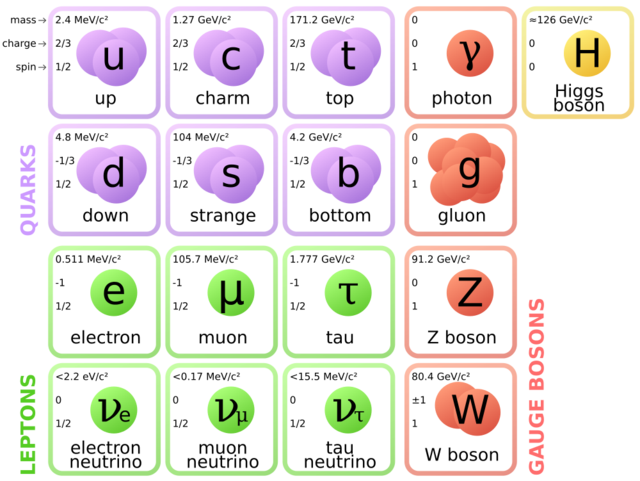
\includegraphics[width=0.50\textwidth]{Figures/Chapter1/SMParticles.png}
\caption{The 17 elementary particles, including 6 leptons, 6 quarks, 4 gauge bosons, and the Higgs boson, and their basic properties, such as mass, electric charge, spin, in the Standard Model of Particles Physics are shown above.}
\label{fig:SMParticle}
\end{center}
\end{figure} 


There are 19 parameters in the Standard Model: 6 quark masses, 3 lepton masses, 3 coupling strengths, 4 angles in the Cabibbo?Kobayashi?Maskawa Matrix, Higgs mass, vacuum expectation value, and QCD vacuum angle. These parameters are determined from the experiments. Physicists perform calculations based on the Standard Model and predict the cross section of different processes in high energy physics experiments. Since it is proposed in the 1970s, the Standard Model has been tested extensively in countless high-energy physics experiments. Its prediction holds for all of them with very few exceptions. The Standard Model consists of two sectors: the Electroweak theory (EW) and Quantum Chromodynamics (QCD). The Lagrangian of the Standard Model can be written as the sum of EW and QCD: $\mathcal{L_{SM}} = \mathcal{L_{EW}} + \mathcal{L_{QCD}}$ 


\section{Quantum Chromodynamics}

\subsection{QCD Lagrangian}

QCD, a non-abelian gauge theory with $SU(3)$ symmetry, is the theory for the strong interaction between quarks and gluons. The QCD Lagrangian is shown as follows:


\begin{equation}
\mathcal{L_{QCD}} = \bar \Psi^i i (\slashed{D})_{ij} \Psi^j - m  \bar \Psi^i \Psi_i - \frac{1}{16\pi^2} G^{\mu\nu}_{a}G_{\mu\nu}^{a}
\end{equation}

Where 

\begin{equation}
\slashed{D} = \gamma^\mu \partial_\mu - i g_s \frac{\lambda}{2}  \gamma^\mu A_\mu
\end{equation}

\begin{equation}
G^{\mu\nu}_{a} = \partial^\mu A^\nu_{a} - \partial_{\nu} A^\mu_{a} + g_s f_{abc} A^\mu_b A^\nu_c 
\end{equation}

Here, $\lambda$ are the Gell-Mann Matrices. $f_{abc}$ is the structure of constant of $SU(3)$. $A^\mu$ is the eight gluon field. $g_s$ is the strong coupling constant. The color indices $i$ and $j$ run from 1 to 3, which stands for 3 colors: red, blue, and green. The gluon field indices $a$, $b$, and $c$ run from 1 to 8, standing for the 8 gluon state (Gluon octet as the combination of 3 color and 3 anticolor: $3 \times \bar 3 = 1 \oplus 8$) living in the adjoint representation of $SU(3)$ of color.  



\subsection{Asymptotic Freedom}

The running of the strong coupling constant $\alpha_s = \frac{g_s^2}{4\pi}$ according to the 1-loop calculations in the renomalization theory \cite{QCDRunning} is shown as follows

\begin{equation}
\alpha_{s} (Q^2) = \frac{12\pi}{(11 N_{c} - 2 N_{f}) \ln(\frac{Q^2}{\Lambda_{QCD}^2})}
\end{equation}

We can see that as the energy scale increases, the coupling strength of the strong interaction decreases. This is in contrast to QED where the electromagnetic coupling strength increases as the energy scale increases. In the ultra-violate limit $Q^2 \rightarrow \infty$ and $\alpha_{s} \rightarrow 0$, quarks and gluons behave like free particles. This feature in QCD is called Asymptotic Freedom \cite{QCDAsym}. Meanwhile, in the infrared limit, the strong coupling constant increases. Near the $\Lambda_{QCD} \simeq$100 MeV, the strong coupling is greater than 1, where the perturbative expansion of QCD breaks down. Experimentally, physicists measure the strong coupling constant at different energy scales from different experiments at different colliders. Figure~\ref{QCDCoupling} \cite{AlphaTheoEx} shows the running of strong coupling constant in experiment and comparison with the theoretical calculations 

\begin{figure}[hbtp]
\begin{center}
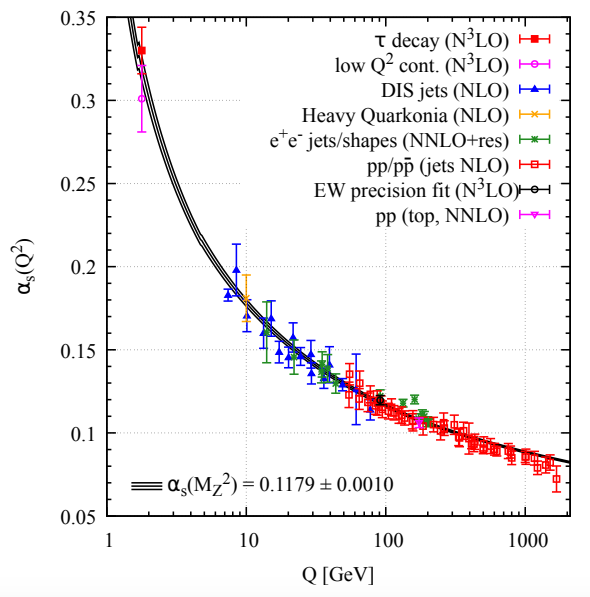
\includegraphics[width=0.50\textwidth]{Figures/Chapter1/QCDCoupling.png}
\caption{The running of the strong coupling constant $\alpha_s$ in different experiments at different energy scale $Q$ and the comparison with QCD calculations are shown above. Image from: \cite{AlphaTheoEx}}
\label{QCDCoupling}
\end{center}
\end{figure} 

An excellent agreement between theoretical predictions and experimental results of the strong coupling constant is observed in Figure~\ref{QCDCoupling}. 

\subsection{Perturbative QCD}

%It is mathematically proven that there is in general no closed form expression for the partition function $Z[J(x)]$ Standard Model Lagrangian under the Quantum Field Theory framework.

So far, there is not any closed form expression yet for the partition function $Z[J(x)]$ Standard Model Lagrangian under the Quantum Field Theory framework.

\begin{equation}
Z[J(x)] = \int \mathcal{D}[\phi(x)] e^{iS + \int d^4 x J(x) \phi(x)}
\end{equation}

Therefore, physicists develop perturbation theory in Quantum Field Theory and apply it to the Standard Model. Physicist perform asymptotic expansions to obtain power series of the coupling constants and approximately calculate the expectation values of the observables to prediction experimental results.

For QCD, ,  perturbation theory is applicable to QCD in high energy and hard scattering processes since the coupling constant is much less than 1. Feynman rules and diagrams are applicable in the matrix element to evaluate the cross section of hard parton-parton scattering. Perturbative QCD (pQCD) calculations have been tested with various experiments such as electron-positron annihilations, deep inelastic electron-proton scatterings, and high energy proton-proton collisions.

\subsection{Non-perturbative QCD}

For soft scattering processes at low energy, the strong coupling constant is greater than 1. Perturbation theory of QCD breaks down. Many low-energy QCD processes such as hadronization and hadron-hadron interactions are non-perturbative. Historically, physicists developed Lattice gauge theory where the spacetime is discretized into lattice with finite size to evaluate the path integrals in the partition function $Z[J(x)]$. Lattice QCD can be applied to calculate the mass of the proton \cite{LQCDProtonMass}. Aside from Lattice gauge theory, effective theory is also to study non-perturbative QCD. For example, Chiral Perturbation Theory, where a low-energy effective Lagrangian in degree of freedom of hadrons is constructed by exploiting the approximate chiral symmetry while preserving other symmetries of parity and charge conjugation, has achieved some success to study pion-nucleon scattering \cite{ChiPT}. Non-perturbative QCD has achieved many successes in hadronic physics. Currently, some novel developments applying non-perturbative QCD to understand nuclear structure and nucleon spin structure are being carried by physicists. For instance, Chiral Perturbation Theory has been applied to study light nuclei structure such as ${}_{3}^{6}Li$ and ${}_{5}^{10}B$ \cite{ChiPTNuclear} and Lattice is employed to investigate nucleon spin structure \cite{LatticeNuclSpin}. 

\subsection{QCD Factorization Theorem}

The QCD factorization theorem states that in events with hadrons as incoming particle involving both hard and soft QCD processes, hard and soft process are mathematically factorized in the cross section computation shown schematically below \cite{QCDFactorization}: 

\begin{equation}
\sigma = PDF \otimes Diagrams \otimes FF
\end{equation}

\begin{figure}[hbtp]
\begin{center}
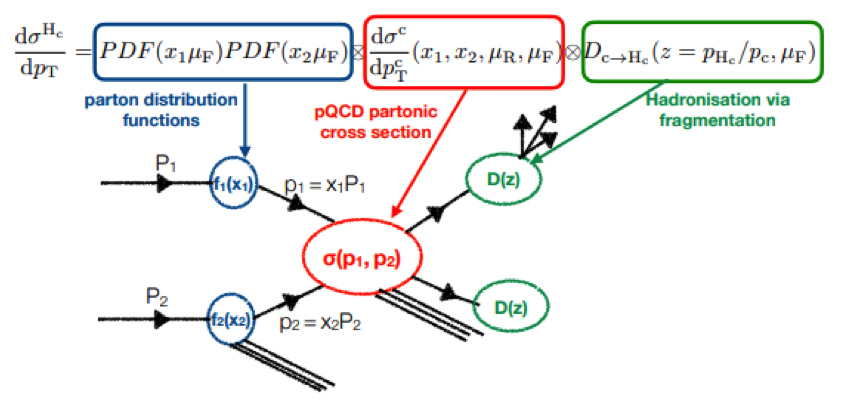
\includegraphics[width=0.75\textwidth]{Figures/Chapter1/QCDFacNew.png}
\caption{The QCD factorization theorem applied to study charm hadron production in a $pp$ collision event involving in soft and hard processes are shown above.}
\label{QCDFacTheo}
\end{center}
\end{figure} 

The hard processes are encoded in the factor of partonic cross sections while the soft processes are measured in experiments. Physicists employ parton distribution function (PDF), defined as the probability of finding a particle with a certain longitudinal momentum fraction $x$ at resolution scale of $\mu^2$, to describe the initial kinematic of partons inside hadrons \cite{PDFRef} and fragmentation function (FF), defined as the probability of a parton turn into a hadron $D_i^h(z)$ for a given energy fraction of the parton $z$ at resolution scale of $\mu^2$, to describe the hadronization process of partons \cite{QCDFFunc}. 

In addition to PDF, we could also define nuclear PDF (nPDF) for \cite{nPDFDef} to describe the parton kinematics inside nucleus. nPDF could be understood as the PDF of nucleons modified by the nuclear environment. Both parton distribution function and fragmentation function are extracted in experiments.

Physicists apply QCD factorization theorem to perform pQCD calculations and compare them with hadron spectra in electron-positron ($e^+e^-$), electron-proton ($ep$), and proton-proton ($pp$) collisions.

\subsection{Color Confinement}

Another feature of QCD as a non-abelian gauge theory is color confinement. The strong force carrier gluon itself is also color charged. Color charged partons, namely quarks and gluons, are never detected in isolation. In experiments, only color neutral hadrons are detected. Currently, the analytic explanation of color confinement is still not yet rigorously proven. The theoretical explanation of color confinement in QCD remains one of the unsolved problem in physics. 

\subsection{Hadronization}

The formation process hadrons from partons is called haronization. Because in experiments we can only measure final state hadrons, in order to study the interactions and dynamics of quarks and gluons during partonic stage from hadron spectra, we also need to understand hadronization mechanisms. However, hadronization is in general non-perturbative and cannot yet be described by first principle QCD calculations. Therefore, physicists make phenomenological models such as the Statistical Hadronization Model \cite{SHM}, Lund String Model \cite{LSM}, Cluster Hadronization Model \cite{CHM}, Quark Coalescence Model \cite{QCM} to study hadronization. Figure \ref{HadMech} schematically shows the hadronization of heavy quarks via fragmentation \cite{JetFrag} and recombination mechanism \cite{QuarkCoal}.

\begin{figure}[hbtp]
\begin{center}
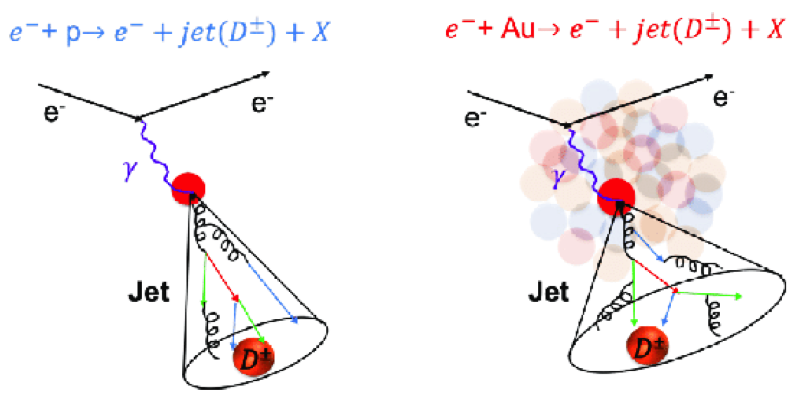
\includegraphics[width=0.48\textwidth]{Figures/Chapter1/FragCartoon.png}
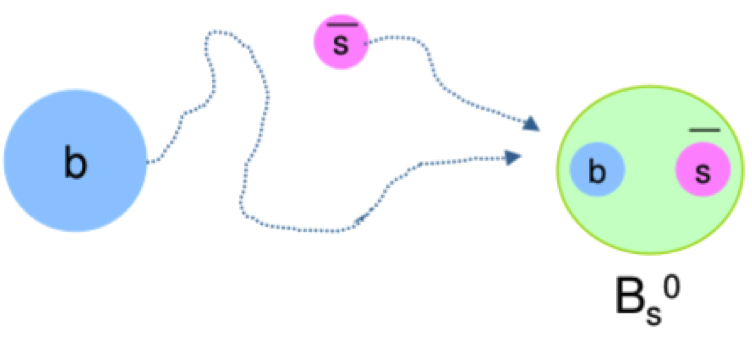
\includegraphics[width=0.48\textwidth]{Figures/Chapter1/CoalCartoon.png}
\caption{The fragmentation process of charms quarks hadronize into $D^\pm$ (left) and the coalescence process of beauty quark combining with a strange quark nearby to form a $B^0_s$ are shown above.}
\label{HadMech}
\end{center}
\end{figure} 


\subsection{Initial State and Final Effect}

In high energy proton-nucleus ($pA$) collisions, protons scatter off nucleons inside nuclei. Assuming QCD factorization still holds, nPDF could be applied to calculate the cross section of particle production. The initial state effects of nuclei including event-by-event geometry fluctuations due to nuclear dynamics \cite{GuntherV3}, nuclear shadowing effect \cite{NuclearShadowing}, EMC effect \cite{EMC} will modify the PDFs of nucleons in nuclei compare to PDFs of nucleons in vacuum. 

In the final state, the struck parton will lose energy from the interaction with the nuclear fragment and modify the final state hadron spectra. Because the parton-hadron interaction is generally non-perturbative, to retain the formula of QCD factorization theorem, the parton FF is modified \cite{CNEEFF}. These initial stage and final stage effects in $pA$ collision are call cold nuclear matter effects. 

\section{Hot QCD}

\iffalse 

\subsection{Initial State and Final Effect}


The development described in the previous section applies in small systems, for example, $e^+ e^-$, $ep$, and $pp$ collisions. In the smallest collision system $e^+e^-$, there is no initial state effect since the electron and positrons are point-like. In $ep$ and $pp$ collision, the initial state effects are encoded in the proton PDF. 

In high energy proton-nucleus collisions, proton scatter off nucleons inside nucleon. Assuming QCD factorization still applies, we can define nPDF to describe the kinematics of quarks inside nucleons of nucleus. We can see that there will be modification to the PDF for a nucleon vacuum due to the nucleon dynamics in the nuclei we can study the cold nuclear matter effects and probe the nPDF. In pA collisions, there many initial state effect depending on the collision $x$ and $Q^2$. For instance, we have nuclear shadowing, gluon saturation, and EMC effect. Both nPDF and the struck parton interact with the nuclear fragment will affect the final state hadron spectra. We call these effects in pA collision as cold nuclear matter effect.
%Hence, in addition to the initial state effect, there are also final state hot QCD matter effects in high energy nucleus-nucleus collisions.  

Initial state CGC 

\fi

\subsection{QCD in Finite Temperature} 

%In high energy, quarks and gluons inside nucleons of the nuclei become relevant to describe the event. As the energy increase, the quark and gluon density of the collision system increases. During the collisions, many quarks and gluons interact with each with in a small volume. 

In a system of dense and energetic quarks and gluons confined in a given size of volume, they scatter with each other and exchange momenta via the strong interaction. Many-body dynamics between quarks and gluons become relevant. In the limit of large number of quarks and gluons, after a sufficiently long period of time, the system eventually converges to the thermal equilibrium state via strong interaction \cite{MLBThermal,ADSCFTThermal,QCDThermal} regardless of its initial states. Therefore, a description based on thermodynamics can be formulated to study such systems \cite{QCDThemDyn}. We call this thermalized many-body system of quarks and gluons to be QCD matter. Therefore, a thermodynamic variable temperature ($\mathbf{T}$) can be introduced to characterize these many-body QCD systems. The study of many-body QCD in finite temperature is called hot QCD. 



\subsection{Temperature Dependence of QCD Static Potential}. 

If we consider two color charged quarks in the limit of infinite mass and are essentially at rest in the lab frame, we can define a QCD static potential between these two quarks due to the strong interaction. In vacuum, such a potential is called ``Cornell Potential'' \cite{Cornell}. The potential as a function of the distance between two quarks is shown as follows:

\begin{equation}
V(r) = -\frac{\alpha_{eff}}{r} + \sigma r
\end{equation}

Here, $\alpha_{eff}$ is the effective strong coupling coupling between the two quarks and $\sigma \simeq 0.184$ GeV/c is the string coupling constant \cite{CornellEquation}. 

Now if we consider a thermalized system in finite temperature $T$, the potential becomes: 

\begin{equation}
V(r) = -\frac{\alpha_{eff}}{r} e^{-m_D r} + \frac{\sigma}{m_D} (1 - e^{-m_D r})
\end{equation}

Here, $m_D \sim g_s T$ is the Debye mass due to Debye color screening effect \cite{CSEff}, which essentially modifies the gluon propagator by inserting a finite mass term: $-i \frac{g^{\mu\nu}}{q^2} \rightarrow -i \frac{g^{\mu\nu}}{q^2 - m_D^2}$. We have observed that as $V(\infty) = \frac{\sigma}{g_sT}$, which is finite for $T>$0. In fact, Equation (2) reduces to the Cornell potential when $T =$ 0. The QCD static potential is shown below in Figure~\ref{QCDPotential} \cite{TDepCornell}


\begin{figure}[hbtp]
\begin{center}
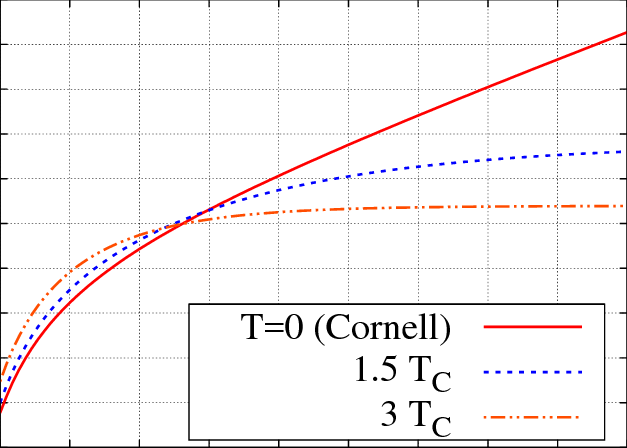
\includegraphics[width=0.55\textwidth]{Figures/Chapter1/QCDPotential.png}
\caption{The QCD potential $V(r)$ from at zero and at finite temperatures as a function of distance $r$ is shown above. Here, the critical temperature $T_c $ = 192 MeV. We can see that the QCD saturates at a finite value at finite temperature. }
\label{QCDPotential}
\end{center}
\end{figure} 


\subsection{Color Deconfinement}

As mentioned in the sections above, at finite temperature, the QCD static potential is screened and color degree of freedom become relevant in the system. As the temperature of the system increases, the quarks and gluon inside color-neutral hadrons will have more available space to move around and start to deconfine \cite{DeconfineTemp}. At some critical temperature $T_c$, quarks and gluons confined in hadrons will melt and form a new state of color deconfined QCD matter, which is called Quark-Gluon Plasma (QGP). The typical temperature of QGP is in the order of a few hundred MeV or about $10^{12}$ K, which is about hundreds of thousands times hotter than the core of the Sun. It is believed that QGP existed in the early universe several microsecond after the Big Bang \cite{QGPUniverse}. Cosmologically, the research on QGP will help us envision the quark epoch and study quark-hadron phase transition to understand the history of the universe \cite{QHPhase}. 

%There are some interesting QCD phenomenologies involving temperature as listed in the following subsections.

%Hot applies in AA collision where a thermalized system is created. 

\subsection{QCD Phase Diagram}

Similar to form everyday matters such as metal, water, wood, glass, and plastic, which are formed by electromagnetic interaction and could all be described macroscopically by equations of states that are parameterized by thermodynamic variables. 
\iffalse Figure~\ref{QEDPhaseDiagram} shows the phase diagram of water ($\mathrm{H_2O}$) at different temperature and pressure:

\begin{figure}[hbtp]
\begin{center}
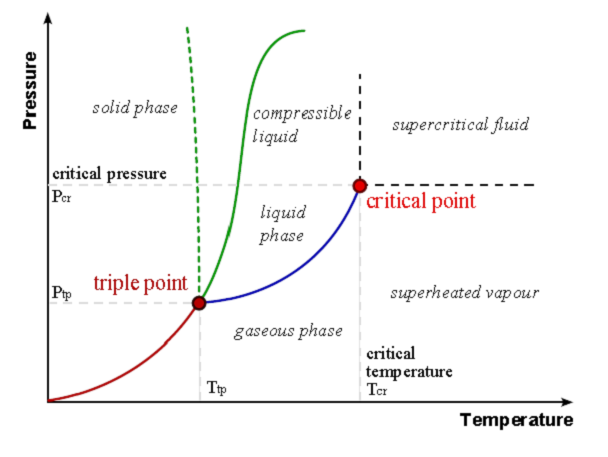
\includegraphics[width=0.45\textwidth]{Figures/Chapter1/WaterPhaseDiagram.png}
\caption{The P-T diagram of water in gas, liquid, solid phases is shown above.}
\label{QEDPhaseDiagram}
\end{center}
\end{figure} 

 
 \fi
Similarly, thermodynamical variables, for instance temperature ($\mathbf{T}$) and baryon chemical potential ($\mu_{B}$) can be introduced to characterize the equation of state of QCD matter formed via the strong interaction between many quarks and gluons. %Similarly, QCD matter is the matter formed by numerous quarks and gluons via the strong interaction and can also be describe by equations of states. L
Like our everyday matter which has gas, liquid, and solid phases at different pressure and temperature, QCD matter also has different phases at different temperature and baryon chemical potential. and can be describe by QCD phase diagrams. Figure~\ref{QCDPhaseDiagram} shows the QCD phase diagram at different temperature and baryon chemical potential:

\begin{figure}[hbtp]
\begin{center}
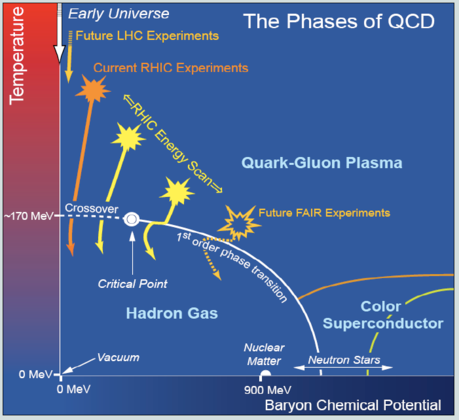
\includegraphics[width=0.60\textwidth]{Figures/Chapter1/QCDPhaseDiagram.png}
\caption{The theoretical QCD phase diagram of different QCD matter, including hadron resonance gas, quark-gluon plasma, neutron star, and color superconductor, as function of temperature and baryon chemical potential is shown above. The solid line indicates the conjecture of first order phase transition between quark-gluon plasma and hadron gas while the dash line is a smooth crossover. Thermodynamically, a critical points must exist in the boundary of smooth crossover and first order phase transition.}
\label{QCDPhaseDiagram}
\end{center}
\end{figure} 

We consider a system of free up and down quarks, antiquarks and gluons in temperature $T$ and baryon chemical potential $\mu_B$. According to MIT Bag Model \cite{MITBag}, its equation of state is given by

\begin{equation}
\epsilon(T,\mu_B) = \frac{37\pi^2}{30} T^4 + \frac{\mu_B^2}{3}T^2 + \frac{\mu_B^4}{54\pi^2} -  \mathcal{B}
\end{equation}

\iffalse
\begin{equation}
\epsilon(T,\mu_B) = \frac{37\pi^2}{30} T^4 + \frac{\mu_B^2}{7}T^2 + \frac{\mu_B^4}{161\pi^2} -  \mathcal{B}
\end{equation}
\fi

Here $p$ is the pressure and $\mathcal{B}$ is the bag constant, which can be understood as the pressure of the vacuum on the quarks and gluons to make them form hadrons with finite volume.

In a system of interacting quarks and gluons at $\mu_B=0$, based on lattice QCD calculations \cite{LatticeQGP}, the reduced energy density $\epsilon/T^4$ as a function of the temperature $T$ is shown below


\begin{figure}[hbtp]
\begin{center}
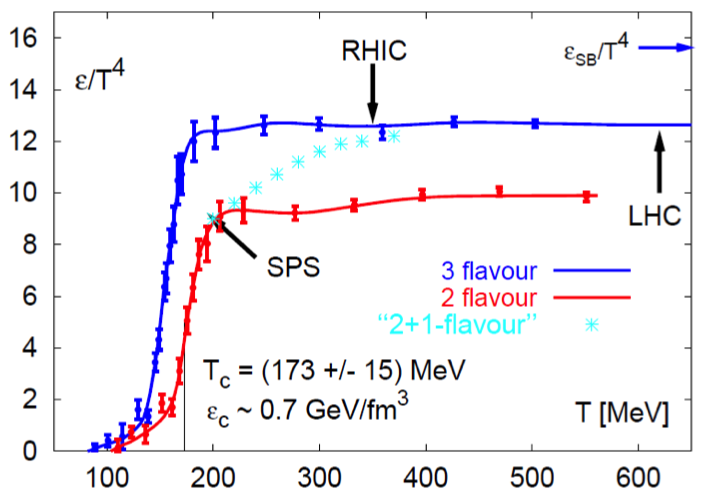
\includegraphics[width=0.60\textwidth]{Figures/Chapter1/LQCDNew.png}
\caption{The reduced energy density $\epsilon/T^4$ as a function of temperature $T$ for different number of flavor scenarios from the lattice QCD calculations (data points) and the interpolation curves are shown above.}
\label{QCDPhaseDiagram}
\end{center}
\end{figure} 


A steep increase of the $\epsilon/T^4$ near the critical temperature at around $T_c  = 173$ MeV is observed, which signals the transition from hadron gas to the QGP \cite{PhaseTrans}. Experimentally, the critical point is estimated to be around $T_c = 175^{+1}_{-7}$ MeV and $\mu_B = (22 \pm 4.5)$ MeV \cite{CriticalPointEX} .






%Phase transition plot from LQCD

%Lattice QCD calculation has shown that.



%In the QCD phase diagram 

%Describe the diagram with QGP, Hadron Gas, and color superconductor.

%Talk a little about phase transition and critical point.

\section{High Energy Nuclear Physics}

Nuclear Physics is the study of atomic nuclei and their constituents and interactions. The typical energy scales of nuclear physics range from MeV to GeV. High Energy Nuclear Physics is a subfield of Nuclear Physics at an energy scale on the order of GeV. Its main goal is to under the physics of QCD matter from various approaches such as collider experiments, astrophysical observations, physics simulations, and theoretical modelings. In this thesis, I will focus on the research of QGP from the experimental approach using high energy heavy-ion colliders.

\subsection{Laboratories}

In laboratories, high energy nuclear physicists accelerate and collide heavy ions (A > 56) at center of mass high energy per nucleon at grater than 1 GeV to create extremely hot and dense conditions and study QGP. Relativistic heavy-ion collision is also known as ``The Little Bang'' compared to ``The Big Bang'' in cosmology \cite{LittleBang}. Historically, many colliders, such as the Alternating Gradient Synchrotron (AGS) at Brookhaven National Laboratory (BNL), in Upton, Long Island, New York and Super Proton Synchrotron (SPS) at European Center for Nuclear Research (CERN) in Meyrin, Switzerland, and GSI at Helmholtz Centre for Heavy Ion Research with both proton-proton and relativistic heavy-ion collision capabilities, have been built and established high-energy nuclear physics research programs. Today, two active colliders facilities, the Relativistic Heavy Ion Collider (RHIC) at BNL and the Large Hadron Collider (LHC) at CERN, are running at a wide range energies with various nuclei species and different impact parameters. In the future, another collider, called Facility for Antiproton and Ion Research (FAIR) running at relatively low energies, is being constructed at Darmstadt, Germany to map the location of the critical point in the QCD Phase Diagram. 

In addition to collider facilities, QGP might also be studied from astrophysical observations. For instance, strange stars, a quark star made of strange quark matter, may come from stable strangelet according to Bodmer--Witten conjecture \cite{SQMReview} or exist in the core of neutron stars under extreme pressure and temperature. It is believe there are several potential strange stars candidates according to telescope observations and gamma ray burst analysis \cite{SS1,SS2,SS3}.

%\subsection{Heavy-Ion Accelerators}

\subsection{Relativistic Heavy Ion Collider (RHIC)}

Located at BNL in Upton, Long Island, New York, United States of America, RHIC is one of the major high energy accelerator facilities and currently the highest energy collider in America. It is a circular collider with a circumference of 3.843 kilometers and can provide proton energy up to 500 GeV and gold ion energy up to 200 GeV \cite{RHICReport}. It was built in 2000 in order to search for a strongly interacting hot and dense state of nuclear matter created under ultra-relativistic heavy-ion collisions, currently known as QGP, with hints from the measurements at AGS and SPS. Moreover, RHIC provides physicists with a wide range of energies and a variety of ion species from proton to deuteron and cooper to uranium to create different sizes of systems at different temperature and baryon densities. In addition, taking the advantage of its highly polarization beam with high luminosity, RHIC has great machine capabilities for cold QCD physics. Figure \ref{RHIC} below shows a sky view of RHIC at BNL:


\begin{figure}[hbtp]
\begin{center}
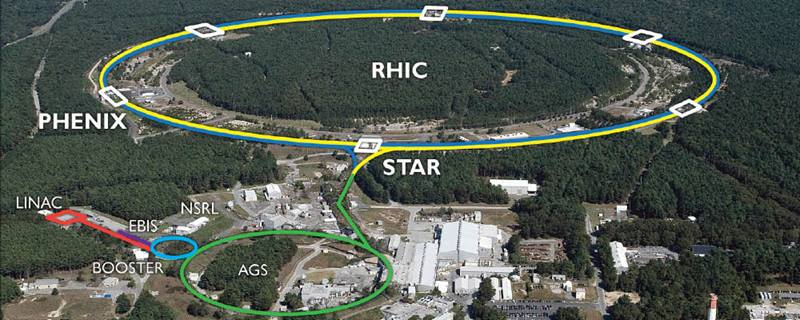
\includegraphics[width=0.85\textwidth]{Figures/Chapter1/RHIC.jpg}
\caption{The view of RHIC at BNL from the sky is shown above. The actual locations of other facilities at BNL, including Linac, Booster, EBIS, NSRL, AGS, and the experiments at RHIC such as, STAR and PHENIX, are also labelled.}
\label{RHIC}
\end{center}
\end{figure} 

Here is how RHIC accelerates charged particle beams to the energy scale of GeV per nucleon through multiple electron stripping and acceleration stages. For instance, if we consider the acceleration of a typical ion source gold (${}^{197}_{79}Au$) ion \cite{AuStripping}., we first use a cesium sputter ion source operated in the pulsed beam mode and point it to the gold metal to produce the $Au^-$ ion \cite{FirstAuSource}. Then, the $Au^{-}$ will undergo a series of electron stripping processes to reach the $Au^{79+}$ ion \cite{RHICStrpDetail}. First, 13 electrons are stripped by the carbon foil in the Terminal Stripping (S1) after the acceleration of tandem Van der Graaf generator to turn $Au^{-}$ into $Au^{12+}$. Then, the $Au^{12+}$ ion will go through the Object Foil (S2) at the second stripping stage and becomes $Au^{31+}$. Next, the $Au^{31+}$ will go through the third stripping station BTA foil (S3) made of aluminum and vitreous carbon between the Booster Synchrotron and AGS and becomes $Au^{77+}$. Finally, two more electrons of the gold ion $Au^{77+}$ are removed at the fourth stripping station ATF foil (S4) made of thin tungsten, located in between the AGS and RHIC. The fully stripped gold ions $Au^{79+}$ will then be injected to the blue and yellow rings at RHIC. For polarized protons, $H^-$ pass a single stripping stage called located in the Booster Synchrotron. The stripping station is called Linac-to-Booster (LTB) stripper made of carbon foils with special geometry and converts polarized $H^-$ to $H^+$. Figure \ref{AccAu} schematically shows the accelerating process of gold ions at RHIC \cite{AuStripRef}

\begin{figure}[hbtp]
\begin{center}
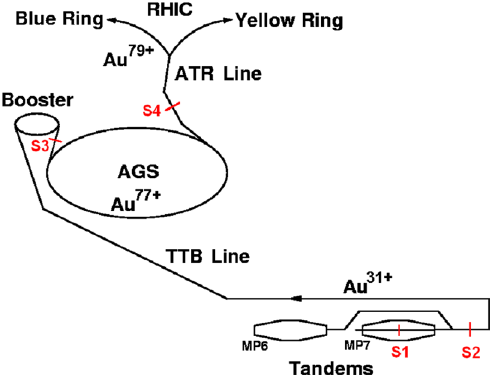
\includegraphics[width=0.45\textwidth]{Figures/Chapter1/AccAu.png}
\caption{The acceleration of gold ions for RHIC is shown above.}
\label{AccAu}
\end{center}
\end{figure} 

At RHIC, we will accelerate the $Au^{79+}$ ions in the superconducting Radio Frequency (RF) cavity under perpendicular electric and magnetic fields until they reach the energies up to about 100 GeV/c per nucleon. Subsequently, we collider them via bunch crossing at the interaction points of the experiments to perform relativistic heavy-ion collisions and study high energy nuclear physics. RHIC usually operates in the first six months of a calendar year. At RHIC, the energy can also be lower where the ion beam collides with ions at a lower energy in the laboratory frame. The STAR experiment at RHIC has already finished beam energy scan and is currently taking data in the fixed target program. 

%RHIC Versatile Machine - Energy + species 

\subsection{Large Hadron Collider (LHC)} 

Located at the border between Switzerland and France, LHC is one of the major high energy accelerator facilities in Europe and currently the highest energy collider in the world. It is a circular collider with a circumference of 26.7 kilometers and can provide proton energy up to 14.0 TeV and lead ion energy up to 5.02 TeV \cite{LHCReport}. It was built in 2008 with the main purpose to discover the Higgs Boson, perform precision measurements on SM, and search for Physics beyond SM. Due to its high energy ion capabilities, high energy nuclear physicists also use the existing general purpose detectors designed for high energy particle experiments at the LHC to conduct research on relativistic heavy-ion physics. LHC ion physics runs usually start at the end of the year and lasts for about a month. The photo taken from the sky to picture LHC is shown in Figure \ref{LHC}:

\begin{figure}[hbtp]
\begin{center}
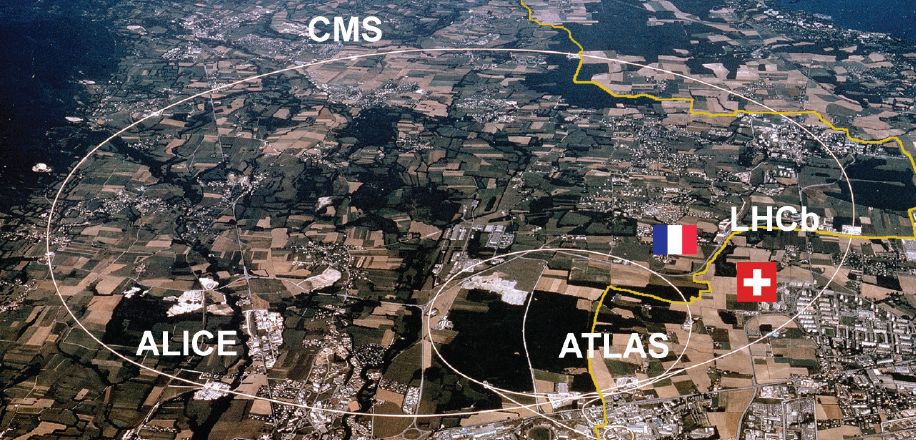
\includegraphics[width=0.85\textwidth]{Figures/Chapter1/LHC.png}
\caption{The sky view of LHC at CERN is shown above. The actual locations of the experiments at the LHC: ATLAS, CMS, ALICE and LHCb, as well as the French-Swiss border, are also displayed.}
\label{LHC}
\end{center}
\end{figure} 

CERN usually uses is lead ${}^{208}_{82} Pb$ ions, which are stable and approximately spherical. In the 2017 ion physics run, it also used the xenon ${}^{131}_{52} Xe$. Currently, there is also a discussion of potential future usage of lighter ions such as oxygen ${}^{32}_{16} O$ \cite{OORun}. Similar to RHIC, the lead ions at the LHC also undergo a series of stripping processes using stripping foils in to order to become partially ionized $Pb^{81+}$ \cite{LHCStrip}. Also, the lead ions pass a series of energy boosting before reaching to the desired energies at the LHC. Lead ions start from a source of vaporized lead and enter Linac 3 before being collected and accelerated in the Low Energy Ion Ring (LEIR) at the energy from 4.2 MeV to 72 MeV. Then, the lead ions will be injected to Proton Synchrotron (PS) to boost their energies. Next, they are sent to the Super Proton Synchrotron (SPS). Finally, the lead ions are injected to the LHC and increase their energies to TeV scale in two LHC rings with the RF cavity \cite{LHCReport}. Finally, the energetic lead ion beams from two LHC rings will collide with a small crossing angle at the interaction points of the LHC experiments. The CERN accelerator complex is shown schematically in \ref{CERNAccComplex} 


\begin{figure}[hbtp]
\begin{center}
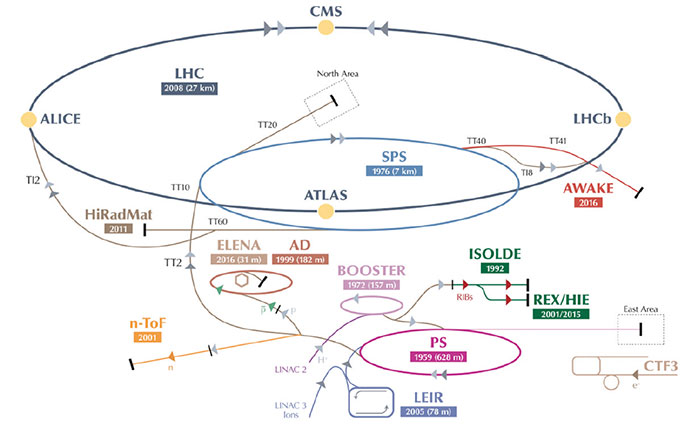
\includegraphics[width=0.65\textwidth]{Figures/Chapter1/CERNAccComplex.jpg}
\caption{The schematic overview of CERN accelerator complex with the accelerators labelled is shown above. Proton and lead ions are accelerated using these facilities and boost their energies to the TeV scale.}
\label{CERNAccComplex}
\end{center}
\end{figure} 

After Run III, LHC will upgrade to high-luminosity (HL) LHC and allows physicists to collect huge datasets, which is crucial to for precision measurements in heavy-ion physics program. Because the beam energy at the LHC is higher than RHIC, the QGP created at the LHC has a higher temperature and a smaller baryon chemical potential than the one created at RHIC.  

\subsection{High Energy Physics Coordinates}

As mentioned in the previous section, heavy-ion is in general highly relativistic. Therefore, Lorentz transformation will be relevant in our studies. In Cartesian coordinates $x^\mu = (t,x,y,z)$, under Lorentz transformation, if we boost the system by a speed $\beta$ in the $+z$ direction. The Lorentz gamma factor will be given by $\gamma = \frac{1}{\sqrt{1 - \beta^2}}$. The four vector $x^\mu \rightarrow x'^\mu$ transforms as follows

\begin{align}
   \begin{bmatrix} 
           t' \\
           x' \\
           y' \\
           z' \\
         \end{bmatrix} =
             \begin{bmatrix} 
             \gamma  & 0  & 0 & - \gamma \beta \\ 
            0 & 1 & 0 & 0 \\ 
             0 & 0 & 1 & 0 \\
             - \gamma  \beta & 0 & 0 &  \gamma \\
	\end{bmatrix} 
	  \begin{bmatrix} 
           t \\
           x \\
           y \\
           z \\
	\end{bmatrix}
\end{align}

The equation above is called the Lorentz Transformation. It is an orthogonal transformation preserving the Minkowski metric tensor $diag(1,-1,-1,-1)$ using particle physicists conventions.


Nowadays, heavy-ion detectors usually have $2\pi$ angular coverage in the transverse direction with some finite longitudinal acceptance along the beam line. They are essentially cylindrically symmetric. Hence, it is convenient and sensible to choose a cylindrical coordinate system and use Lorentz invariant kinematic variables. In general, we define the beam direction to be the z-direction of the coordinate system. Fort the standard cylindrical coordinates in the position space, the Lorentz four-vectors is $(t,x,y,z) \rightarrow (t, r, \phi, z)$. 


The relativistic coordinate system for our analysis is shown below in Figure \ref{HICoordinates}. 

\begin{figure}[hbtp]
\begin{center}
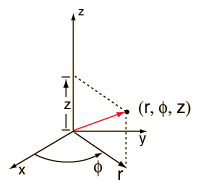
\includegraphics[width=0.40\textwidth]{Figures/Chapter1/PosCylindrical.png}
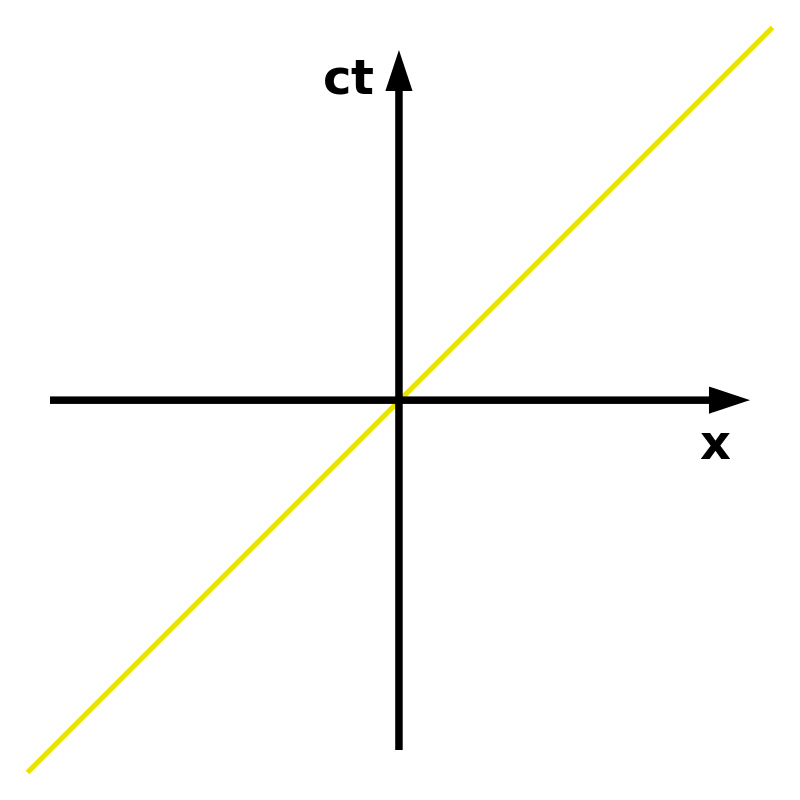
\includegraphics[width=0.40\textwidth]{Figures/Chapter1/STDiagram.png}
\caption{The cylindrical coordinate system in the position space (left) and the space time diagram (right) for relativistic heavy-ion physics analysis are shown above.}
\label{HICoordinates}
\end{center}
\end{figure} 


Thus, in the momentum space, we can use $p^\mu = (E,p_x, p_y, p_z) \rightarrow  (E,p_T, \phi, p_z)$ 

\begin{equation}
p_T = \sqrt{p_x^2 + p_y^2}
\end{equation}

\begin{equation}
\phi = \arctan(\frac{p_y}{p_x})
\end{equation}

We also define rapidity $y$, a relativistic version of velocity that can be convenient add to the boost.

\begin{equation}
y = \frac{1}{2} \ln \frac{E+p_z}{E-p_z}
\end{equation}


Experimentally, we also use pseudo-rapidity $\eta$, which is more directly connected to the detector measurements assuming ultra-relativistic limit kinematics ($E \rightarrow p$). The definition of pseudo-rapidity $\eta$ is shown as follows:

\begin{equation}
\eta =  - \ln \tan(\frac{\theta}{2})
\end{equation}

Here $\theta$ is the angle labelled in the left of Figure \ref{HICoordinates}. Particularly, $y = 0$ and $\eta = 0$ when $p_z = 0$. In addition, boosting by a speed $\beta$ in the longitudinal z-direction, we found that the rapidity simply shift by a const number $y' = y + \tanh \beta$. We should note that the cylindrical coordinates ($p_T$,$\phi$, $p_z$) are perfectly orthogonal while ($p_T$,$\phi$, $y$) or ($p_T$,$\phi$, $\eta$) are not.

For general collider experiments, two particles are moving toward each other with four-momenta $p_1^\mu$ and $p_2^\mu$ and interact with each other. It is also very convenient to use the Mandelstam variables $s, t, u$ in our studies. They are defined as follows

\begin{equation}
s \equiv (p_1 + p_2)^2
\end{equation}

\begin{equation}
t \equiv (p_1 - p_2)^2
\end{equation}

\begin{equation}
u \equiv (p_1 - p_3)^2
\end{equation}


In the center of mass frame, the momentum three vector follows $\vec{p_1} = -\vec{p_2} = \vec{p}$. Therefore, $p_1^\mu = (E, \vec{p})$ and $p_2^\mu = (E, -\vec{p})$. Hence, $s \equiv (p_1 + p_2)^2$ = $4E^2$ = $E_{CM}^2$. Hence, the center of mass energy of the collision system could be represented by the Mandelstam variable $\sqrt{s}$: $E_{CM} = \sqrt{s}$.


%\subsection{Heavy-ion Physics Detectors}

\subsection{Stages of Heavy-Ion Collisions}

In high energy heavy-ion collisions, both Electroweak and QCD processes occur in each event and contribute to the total cross section. We classify the events with elastic and inelastic reaction processes. For elastic processes, two nuclei scatter mainly electromagnetically with each via photon exchange without breaking themselves up or losing energy. For inelastic scattering, we classify diffractive and non-diffractive disassociation processes. In diffractive dissociation processes, the two nuclei may be slightly excited and lose a relatively small fraction of their energies, and produce relatively small number of particles. On the other hand, in non-diffractive dissociation processes, the nuclei lose a substantial fraction of their energies and produce a large number of particles \cite{CYWong}. 

Therefore, in events with significant contribution from non-diffractive dissociation, the interaction between two nuclei has multiple stages including both perturbative and non-pertubative QCD processes. We can define stages of heavy collisions and study the details of each stage. There are five stages: initial state of two highly Lorentz contracted nuclei before the collision, the very early pre-equilibrium stage when hard scatterings between partons inside nuclei begin, the rapid expansion of the fireball when the thermally and chemically equilibrated QGP is created, the hadronization stage after QGP expands and cools down, and the freeze-out stage when the inelastic scattering processes cease.


\begin{figure}[hbtp]
\begin{center}
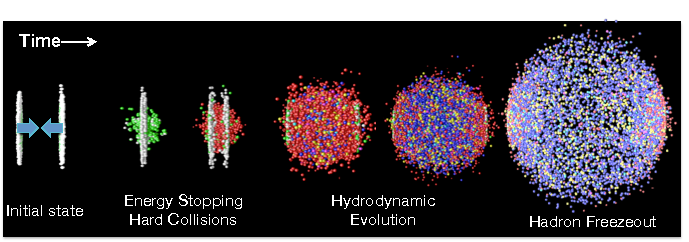
\includegraphics[width=0.80\textwidth]{Figures/Chapter1/Heavy-Ion-Process.png}
\caption{An event of a typical heavy-ion collisions event with different stages as time evolves is shown above.}
\label{HeavyIonStages}
\end{center}
\end{figure} 

\begin{figure}[hbtp]
\begin{center}
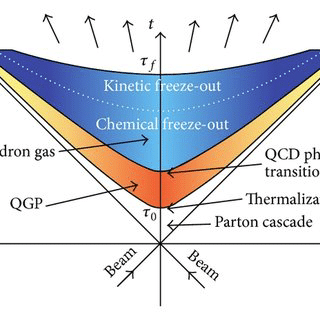
\includegraphics[width=0.45\textwidth]{Figures/Chapter1/HICSTEvolve.png}
\caption{The space-time evolution of heavy-ion collisions is shown above. It consists of four stages: initial state before the collision, early stage of hard scattering processes, the hydrodynamic expansion of QGP, hadronization after QGP expands and cools down, and the freeze-out stage, first chemical freezeout when the particle species no longer change, and finally kinetic freezeout when the elastic scattering processes ceas.}
\label{HICEvolution}
\end{center}
\end{figure} 

Theoretically, many phenomenological models such as Ultra-Relativistic Quantum Molecular Dynamics (UrQMD) and A Multi-Phase Transport Model (AMPT) are developed to describe relativistic heavy-ion collisions. 


\subsection{Global Event Observables}

Globally, we can define some physical quantities in heavy-ion collisions to generally characterize each event. Heavy-ion physicists define the impact parameter, centrality, number of participants, number of binary nucleon-nucleon collisions, and event multiplicity. We will discuss all of them below.

\textbf{Impact Parameter:} Prior to heavy-ion collisions, similar to other collider experiments, each event are prepared with the same unpolarized incoming particles with the same center of mass energy. Therefore, the incoming state $\ket{i}$ is used for each event. However, different from $e^+ e^-$ and $pp$ collision, in heavy-ion physics, we introduce another parameter called the impact parameter denoted $b$ to the transverse distance between center of two nuclei to classify the events. Therefore, the incoming state can be rewritten as  $\ket{i (b)}$. Figure \ref{IPHIColl} shows the definition of impact parameter in heavy-ion collision \cite{IPHICText}.

\begin{figure}[hbtp]
\begin{center}
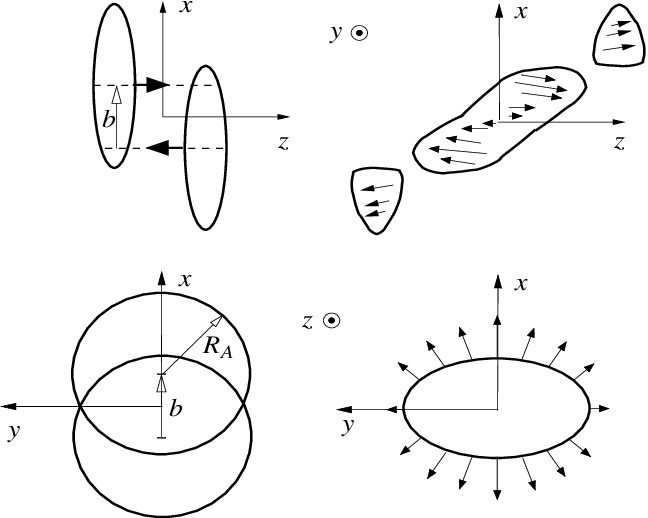
\includegraphics[width=0.60\textwidth]{Figures/Chapter1/IPHIColl.png}
\caption{The definition of impact parameter $b$ in heavy-ion collisions, the of overlapping interaction region, and the break up remnants of the two nuclei, which is called spectator, moving in the z-direction are shown above. An almond shape of the nuclear interaction region, which results in the azimuthal anisotropic emission of final state particles, is seen in heavy-ion collisions.}
\label{IPHIColl}
\end{center}
\end{figure} 


\textbf{Number of Participants:} Right at the end of heavy-ion collisions after two nuclei pass through each other, we can define the number of participants denoted $N_{part}$. The number of participants is essentially equivalent to the number of participating nucleons. The smaller the impact parameter, the more overlap volume between two nuclei, leading to a larger number of number of participating nucleons in the collision. The nuclear interaction system size is determined by the number of participating nucleons. However, due to event-by-event nuclei geometry fluctuations caused by the motion of nucleons inside nuclei \cite{GuntherV3}, it is more proper to say that the average number of participant $\langle N_{part} \rangle$ is related to the impact parameter.

\textbf{Number of Binary Nucleon-Nucleon Collisions:} In addition to $N_{part}$, we can also define another quantity that characterizes the detailed interaction in the events at rather hard scales. The number of binary nucleon-nucleon collisions, denoted $N_{coll}$, is also related to the impact parameter. At higher energy, nucleons inside nuclei become the relevant degree of freedom to describe the cross section. We could treat the collisions of two nuclei as the superposition of the collisions between nucleons inside the nuclei. Since binary nucleon-nucleon collision has a rather small cross section, it dominates the total nucleon-nucleon cross section according to binomial principle. Higher order effects, such as ternary nucleon-nucleon collisions, are negligible. The Glauber model \cite{CentPlot} is developed to study the relationship between $b$, $N_{part}$, and $N_{coll}$ in nuclei collisions and will be discussed in the following subsection.


\textbf{Centrality:} Experimentally, it is difficult to directly measure the impact parameter of each collision. Therefore, we define another physical quantity called centrality to characterize the impact parameter. The centrality ($C$) is defined as the fraction of the total nuclear interaction cross section: $C = \int^b_0 \frac{d\sigma}{dx} dx$ . Centrality is expressed in terms of percentage \cite{CentDef}. It is related to the quantity: $\frac{\pi b^2}{4\pi R_A^2}$ where $R_A$ is the radius of a nuclei defined above in Figure \ref{IPHIColl}. When the impact parameter between two nuclei is 0, the centrality is at 0\%. When the impact parameter between two nuclei is 2$R_A$, the centrality is 100\%. There is also a relationship between the centrality and the average number of participants. Heavy-ion experimental measurements are in general presented in terms of centrality or average number of participants. Experimentally, we look at the number of tracks and cluster energies of calorimeters at the forward direction, for instance, the forward hardonic calorimeters, to estimate the centrality \cite{ALICEZDC,CMSZDC,ATLASZDC}. 


\textbf{Virtuality:} Similar to deep inelastic scattering, we can also define the virtuality $Q^2$, which is the momentum transfer between the two nucleons in nucleon-nucleon collisions. To generate nucleon-nucleon collision event in Monte Carlo (MC) simulation, we used $\hat p_T$, defined as the transverse momentum of the hard subprocess, which is a quantity related to $Q^2$, developed by the high energy theory group of Lund University.


\textbf{Event Multiplicity:} We can also define the event multiplicity by counting the number of final state charged particles to quantify the activity of the event. Event multiplicity can be denoted as $N_{trk}$, number of tracks in the event, which is approximately proportional to the number of charged particle denoted as $N_{ch}$. Figure \ref{CentDefPlot} shows the correlation between the number of participants, their cross section, and the impact parameter in heavy-ion collisions, defining the centrality classes \cite{CentPlot}.


\begin{figure}[hbtp]
\begin{center}
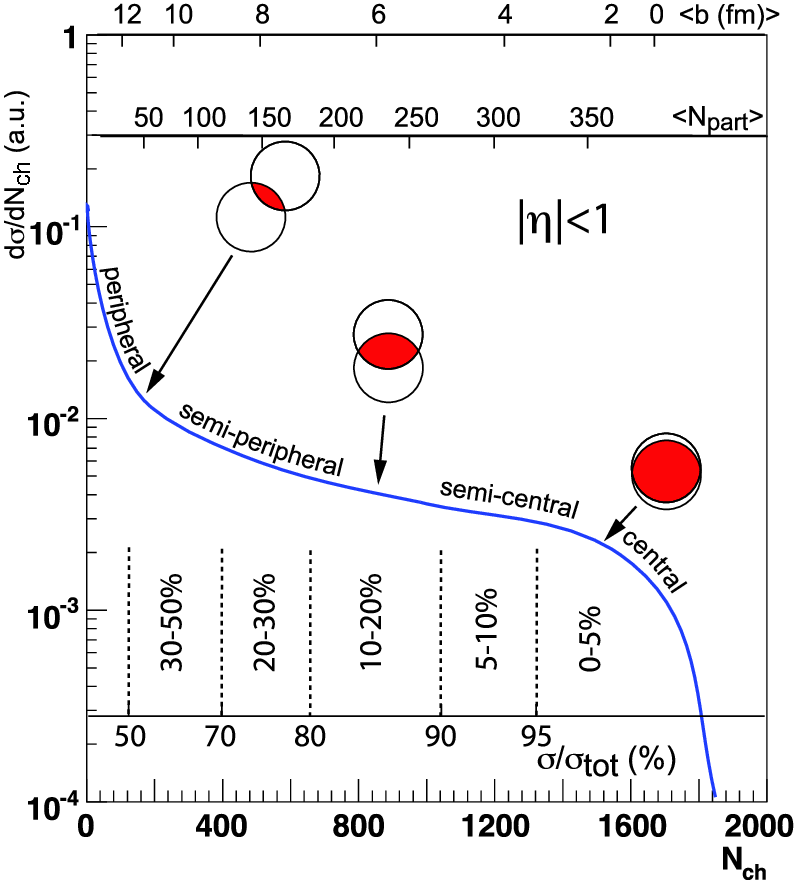
\includegraphics[width=0.55\textwidth]{Figures/Chapter1/CentDefPlot.png}
\caption{The plot showing relationship among number of charged particle, $N_{ch}$, related to the number of participants $N_{part}$, the differential cross section $\frac{d\sigma}{dN_{ch}}$, and the centrality, according to the Glauber Model calculations, is shown above.}
\label{CentDefPlot}
\end{center}
\end{figure} 


The initial global parameters such as the collisions energy, impact parameter, collision nuclei species, and polarization can be treated as knobs for high energy nuclear physicists to play with in order to study relativistic heavy-ion collisions and create strongly interacting systems with different sizes, chemical potentials, and temperatures in the QCD phase diagram. Figure \ref{STAREvtDisplay} shows an event display of thousands of tracks from a central Au + Au collision event at 200 GeV recorded by the Time Projection Chamber (TPC) of the STAR experiment at RHIC.


\begin{figure}[hbtp]
\begin{center}
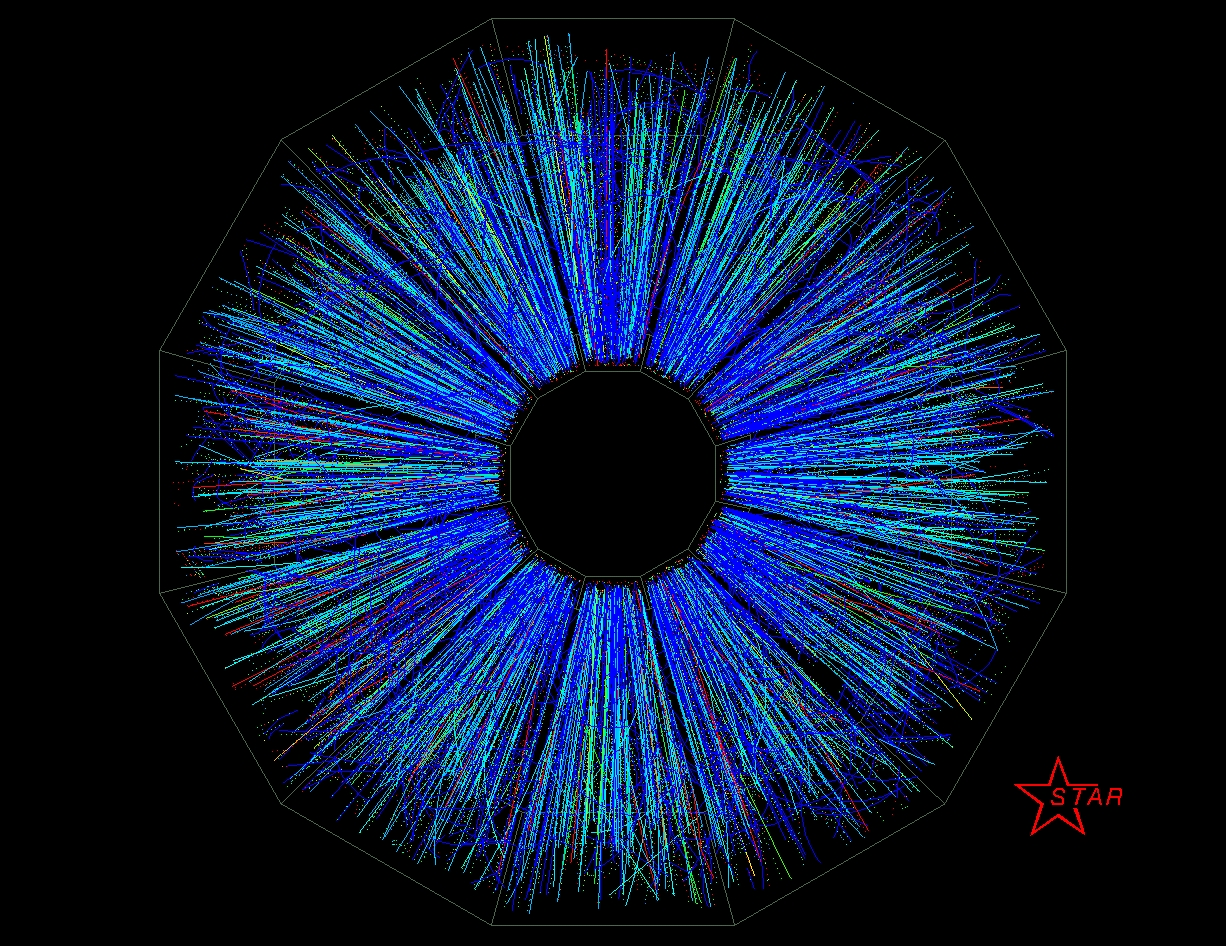
\includegraphics[width=0.50\textwidth]{Figures/Chapter1/STAREvtDisplay.png}
\caption{Two gold ions collide head-on in the STAR detector. The event with reconstructed tracks of final state particles are display by STAR TPC shown above. Image from \cite{STARTPC}}
\label{STAREvtDisplay}
\end{center}
\end{figure} 



\subsection{Glauber Model}

The Glauber Model, named after physicist Roy Glauber \cite{Glauber}, was originally developed to address high energy scattering problems with composite particles in the optical limit where optical theorem is applicable \cite{Optical1,Optical2}. It is a model describing two composite objects collider inelastically with each other and decompose the total cross section to the cross section of collision between two point objects. The Glauber Model can be applied to study nucleon-nucleus (N-A) and nucleus-nucleus (A-B) collisions with nucleon-nucleon (N-N) collisions and determine relationship between the global observables mentioned in the previous subsection.    

If we consider a spherically symmetric nucleus, the nuclear charge density can be described $\rho(r)$ by the Fermi distribution with three parameters below

\begin{equation}
\rho(r) = \rho_0 \frac{1 + w(r/R)^2}{1 + \exp({\frac{r-R}{a}})}
\end{equation}

The equation above is called the Wood-Saxon density formula. According to the Glauber Model \cite{Glauber}, the N-N inelastic cross section is denoted as $\sigma_{in}^{NN}$ and the effective thickness function of a nucleon is defined as a function of impact parameter in the transverse direction: $T(\vec{b})$. It is defined as follow

\begin{equation}
T(\vec{b}) =  \int \rho(\vec{b},z) dz 
\end{equation}

It is normalized to unity: $\int^{R_A}_0 T(\vec{b}) d^2b = 1$. $T(\vec{b})$ essentially depends on density of the nucleus $r(b)$. %If the nucleus is a uniform cylinder and the collide on its circular face along its height, then $T(\vec{b})$ will be a constant. 
Therefore, the probability that a nucleon collides with a nucleon inside the nucleus is given by $\sigma_{in} T(\vec{b})$. Therefore, the probability of $n$ nucleon collisions is given by

\begin{equation}
P_n = {A \choose n} \sigma_{in}^{NN} T(\vec{b})^{n} [1 - \sigma_{in} T(\vec{b})]^{A-n}
\end{equation}

Hence, if we consider a constant fraction of $\mu$ ($0 \le \mu \le 1$) of particle produced after each collisions, we can calculation the average event multiplicity $\langle N(\mu) \rangle$:

\begin{equation}
\langle N(\mu) \rangle = \Sigma_n P_n \Sigma^{n-1}_0 \mu^m =  \Sigma_{n-1} P_n \frac{1 - \mu^n}{1 - \mu} = \frac{1}{1-\mu} \{ 1 - [1 - (1-\mu) \sigma_{in} T(\vec{b})]^A \}
\end{equation}

It turns out that we have the following relationship between $N_{part}$ and $N_{coll}$ with $\langle  N(\mu) \rangle$  \cite{Glauber}

\begin{equation}
N_{part} = \langle N(\mu = 0) \rangle 
\end{equation}

\begin{equation}
N_{coll} = \frac{1}{2} \langle N(\mu = 1) \rangle = A T(\vec{b}) \sigma_{in}^{NN}
\end{equation}

In a more generalized case: A-B collisions, Figure \ref{GlauberRef} shows side view and beam-line view of heavy-ion collision of projectile B on target A


\begin{figure}[hbtp]
\begin{center}
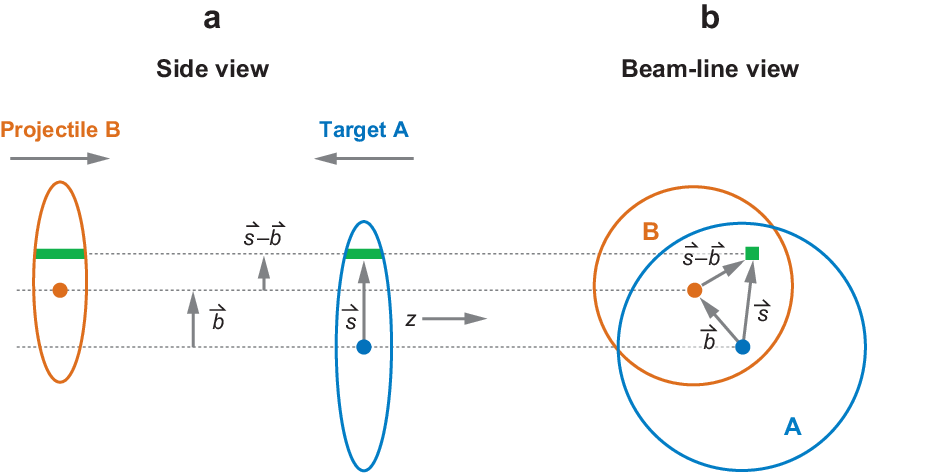
\includegraphics[width=0.65\textwidth]{Figures/Chapter1/GlauDefColl.png}
\caption{The A-B collision with the definition of the impact parameter vector $\vec{b}$ and the distance of nucleon to the center of projectile B $\vec{s}$ are shown above. The distance of the nucleon in B to center of the target A is $\vec{s}-\vec{b}$ according to vector subtraction rule. Here we assume both nuclei A and B are perfect spheres.}
\label{GlauberRef}
\end{center}
\end{figure} 

Using similar ideas \cite{CentPlot}, we could first calculate the effective thickness function $T_{AB}$ as follows:


\begin{equation}
T_{AB}(\vec{b}) = \int T_A(\vec{s}) T_B(\vec{b} - \vec{s}) d^2s 
\end{equation}



Now replacing T($\vec{b}$) in N-A by $T_{AB}(\vec{b})$ in A-B, we can obtain

\begin{equation}
\begin{multlined}
\langle N(\mu) \rangle = \frac{A}{1-\mu} \int_0^b T_A(\vec{s}) \{1 - [1 - (1 - \mu) T_{B}(\vec{b}-\vec{s}) \sigma_{in}^{NN}]\}^A d^2s  \\
  +  \frac{B}{1-\mu} \int_0^b T_B(\vec{s}) \{1 - [1 - (1 - \mu) T_{A}(\vec{b}-\vec{s}) \sigma_{in}^{NN}]\}^B d^2s
\end{multlined}
\end{equation}


To obtain $N_{part}$, evaluate at $\mu = 0$, we get 

\begin{equation}
N_{part} =  A \int_0^b T_A(\vec{s}) \{1 - [1 - T_{B}(\vec{b}-\vec{s}) \sigma_{in}^{NN}]^A\}d^2s +  B \int_0^b T_B(\vec{s}) \{1 - [1 - T_{A}(\vec{b}-\vec{s}) \sigma_{in}^{NN}]^B\} d^2s
\end{equation}

To obtain $N_{coll}$, evaluate at $\mu = 1$, we get

\begin{equation}
N_{coll} = AB T_{AB}(\vec{b}) \sigma_{in}^{NN}
\end{equation}

In a very special case, assume the nuclei are simply perfect rigid sphere with the same radius and collide with zero impact parameter is $b=0$. That is $T_{A} \sigma_{in}^{NN} = T_{B} \sigma_{in}^{NN} = T_{AB} \sigma_{in}^{NN} = 1$, we get 


\begin{equation}
N_{part} = A + B
\end{equation}

\begin{equation}
N_{coll} = AB
\end{equation}

The results above of $N_{part}$ and $N_{coll}$ agree to our expectation. 

The comparison of the Glauber Model with simulations of the $N_{part}$ and $N_{coll}$ as a function of impact parameter $b$ is shown on Figure \ref{NPartandNColl} from the \cite{CentPlot}

\begin{figure}[hbtp]
\begin{center}
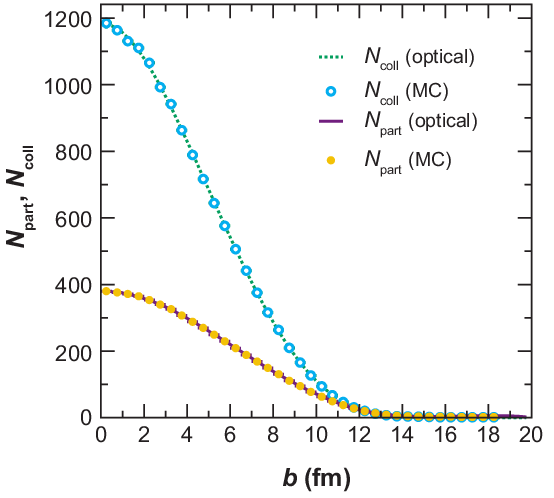
\includegraphics[width=0.50\textwidth]{Figures/Chapter1/NPartandNColl.png}
\caption{The $N_{part}$ and $N_{coll}$ as a function impact parameter calculated from the Glauber Model with optical approximation (lines) and from MC simulations (circles) are shown above. We can see they have almost perfect agreement with each other.}
\label{NPartandNColl}
\end{center}
\end{figure} 


Therefore, we can apply the Glauber model to determine $N_{part}$ and $N_{coll}$ for a given centrality range of AA collision ($T_{AB} \rightarrow T_{AA}$), which will be used in our analysis to obtain the corrected yield. It has been reported that the production of light hadrons, such as pions and kaons, are scaled as $N_{part}$ \cite{NPartScaling} while electroweak bosons, such as W and Z boson, are scaled as $N_{coll}$ \cite{NCollScaling}.

\section{Characterization of Quark-Gluon Plasma}

Equipped with the knowledge and collider technologies of heavy-ion collisions, we are ready to apply them to conduct scientific research on QGP in laboratories. The following subsections will describe the characterization of QGP from its predicted signatures to open questions today, which leads to my thesis research.

\subsection{Signatures}

QGP has been hypothesize long before its discovery as a color deconfined phase of quark matter named ``quark gluon plasma'' \cite{LeonQGP} and will demonstrate some specific benchmarks in experiments to prove the creation of QGP \cite{QGPSignature}. Here, four classic signatures of QGP will be discussed: $J/\psi$ and $\Upsilon$ suppression, jet quenching, elliptic flow, strangeness enhancement.  

\subsection{$J/\psi$ and $\Upsilon$ suppression} 

$J/\psi$ meson, as a type of heavy quarkonia, is bound state of $c\bar c$, made of charm quark and an anti-charm quark, with mass heavier than the $\Lambda_{QCD}$. Therefore, we could approximately treat the interaction between charm and the anti-charm quark with a static the Cornell potential $V(r)$ in the non-relativistic quantum mechanical hamiltonian system \cite{QuarkoniaV}: 

\begin{equation}
\hat H = \hat T + \hat V
\end{equation}

\begin{equation}
\hat H \ket{\psi} = i \frac{\partial}{\partial t}  \ket{\psi} 
\end{equation}

and solve Schrodinger equation the to describe $J/\psi$ mesons in vacuum. As we have seen in Section 1.3.2, with the QGP medium, at a finite temperature $T$, the potential is modified due to color screening effect \cite{QCDString}. The distance between two charm quarks $V(r) \rightarrow \frac{\sigma}{m_D}$, which does not diverge, as $r \rightarrow \infty$. Therefore, the $c \bar c$ system could be unbounded if they have sufficiently high energy. In the field theory picture, this could be understood as the color string breaking between charm and anti-charm quark \cite{CSBQQ}, also known as quarkonia melting \cite{QQMelt}. Hence, with the influence of QGP at $T > 0$, the production cross section of $J/\psi$ will decrease compared to the vacuum at $T=0$. Experimentally, we define an observable to quantify the modification of particle production cross section in $AA$ collision compared to the reference $pp$ collisions normalized by the number of binary nucleon-nucleon collisions $N_{coll}$, which is defined in the previous subsection. We called this observable as nuclear modification factor denoted $R_{AA}$. Mathematically, $R_{AA}$ is defined as follows:

\begin{equation}
R_{AA} =\frac{1}{N_{coll}} \frac{\frac{d^2N_{AA}}{dp_T dy}}{\frac{d^2N_{pp}}{dp_T dy}} = \frac{1}{T_{AA}} \frac{\frac{d^2N_{AA}}{dp_T dy}}{\frac{d^2\sigma_{pp}}{dp_T dy}}
\end{equation}

Therefore, $R_{AA} < 1$ means suppression. $R_{AA} =1$ means no modification. $R_{AA} > 1$ means enhancement. Hence, in experiments, we expect to observe the $R_{AA} < 1$ a suppression of $J/\psi$ production. Figure \ref{JPsiSupp} shows the measurement of fully reconstructed $J/\psi$ at RHIC and LHC \cite{STARJpsi}


\begin{figure}[hbtp]
\begin{center}
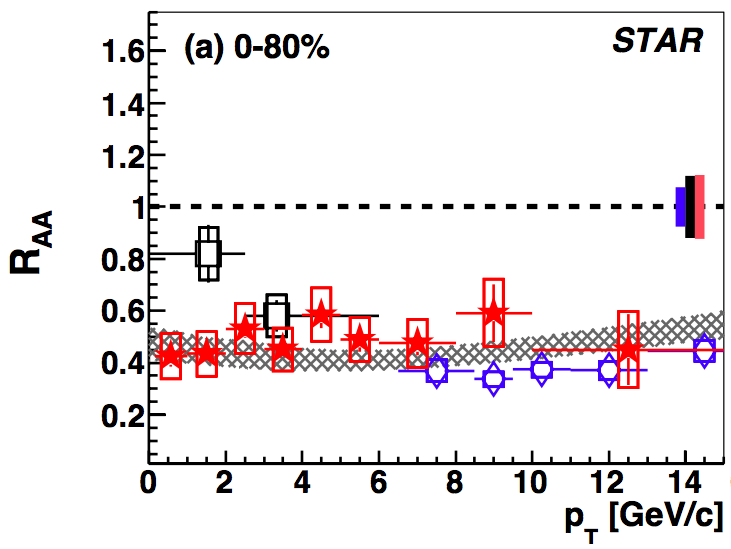
\includegraphics[width=0.47\textwidth]{Figures/Chapter1/STARPt.png}
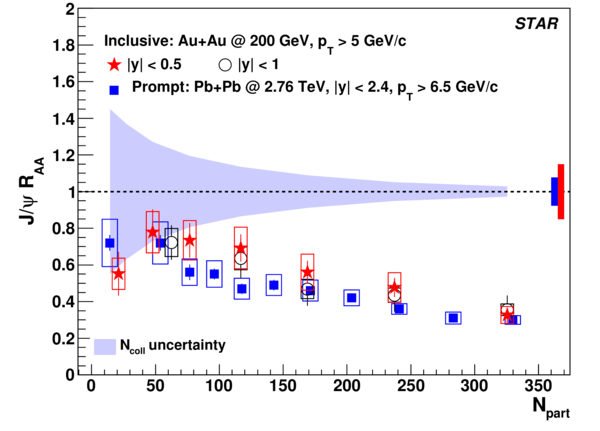
\includegraphics[width=0.487\textwidth]{Figures/Chapter1/STARNPart.png}
\caption{The nuclear modifications factor $R_{AA}$ of fully reconstructed $J/\psi$ as a function of $p_{T}$ (left) and $N_{part}$ (right) measured by the STAR experiment (red data points) at RHIC and CMS (blue diamond data points) and the ALICE (blue circle data points) experiment at the LHC are shown above. We can see that the $J/\psi$ $R_{AA}$ is below 1 for both $p_T$ and $N_{part}$. There is no significant $p_T$ dependence of $J/\psi$ $R_{AA}$. The $J/\psi$ $R_{AA}$ decreases as $N_{part}$ increases, consistent to the increasing creation probability of QGP with larger $N_{part}$.}
\label{JPsiSupp}
\end{center}
\end{figure} 

In fact, we could see that $R_{AA} < 1$ for every data point, which indicates a clear suppression of $J/\psi$ production from experiments at both RHIC and the LHC. However, we should note that the larger $J/\psi$ $R_{AA}$ observed at the LHC compared to RHIC could be explained by regeneration mechanism \cite{JPsiRegen}. %The observation of $J/\psi$ suppression is one of the earliest evidence of the discovery of QGP.

Similarly, we expect to see this in $\Upsilon$, which is made of $b \bar b$. Indeed, they expect to have sequential suppression since 3 $\Upsilon$ states: $\Upsilon(1S)$,  $\Upsilon(2S)$, and $\Upsilon(3S)$, could be observed in experiments. Because the total energy of the $b \bar b$ system or equivalently the rest mass: $m_{\Upsilon(3S)} > m_{\Upsilon(2S)} > m_{\Upsilon(3S)}$, a sequential suppression: $R_{AA}^{\Upsilon(1S)} > R_{AA}^{\Upsilon(2S)} > R_{AA}^{\Upsilon(3S)}$ should be observed if QGP is created. Figure \ref{UpsilonSupp} shows the measurements of fully reconstructed $\Upsilon$ states at RHIC and LHC \cite{STARUpsilonRef,CMSUpsilonRef}

\begin{figure}[hbtp]
\begin{center}
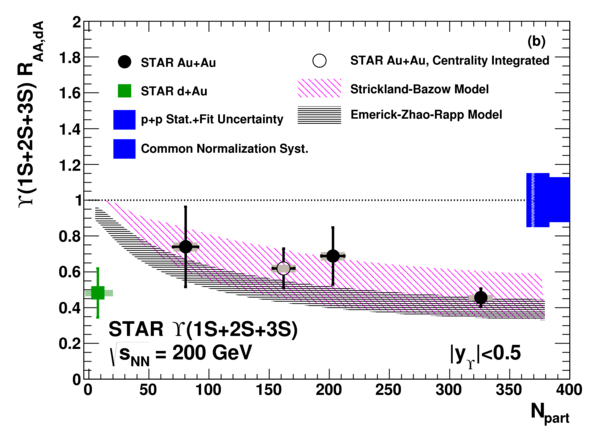
\includegraphics[width=0.52\textwidth]{Figures/Chapter1/STARUpsilon.png}
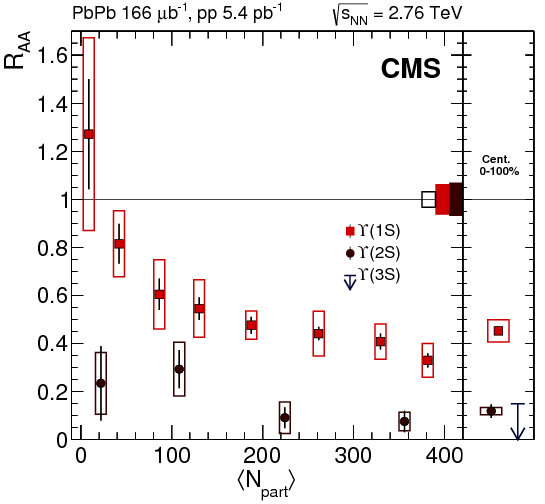
\includegraphics[width=0.40\textwidth]{Figures/Chapter1/CMSUpsilon.png}
\caption{The nuclear modifications factor $R_{AA}$ of fully reconstructed $\Upsilon$ as a function of $N_{part}$ measured by the STAR experiment (left) at RHIC and CMS experiment (right) at the LHC are shown above. We can see that the $R_{AA}$ of the three $\Upsilon$ states are below 1 when $N_{part} > 3$. The $\Upsilon$ $R_{AA}$ decreases as $N_{part}$ increases, consistent to the increasing creation probability of QGP with larger $N_{part}$. In addition, a sequential suppression of $\Upsilon$ $R_{AA}$ is observed by the CMS experiment: $R_{AA}^{\Upsilon(1S)} > R_{AA}^{\Upsilon(2S)} > R_{AA}^{\Upsilon(3S)}$, which agrees with the expectation QGP color screening effect.}
\label{UpsilonSupp}
\end{center}
\end{figure} 


\subsection{Jet Quenching} 

Experimentally, due to color confinement, it is impossible to directly detect and track the energetic partons. Therefore, physicists define jet as a spray of collimated hadrons within a narrow cone initiated from color charged partons. In nuclear and particle physics, jets are used to study the dynamics of partons before hadronization \cite{HERAJET} and understand the properties of QGP. A schematic view of a di-jet production from di-qurark event in electron-positron collider $e^+e^-\rightarrow q \bar q$ is shown below in Figure \ref{dijet}


\begin{figure}[hbtp]
\begin{center}
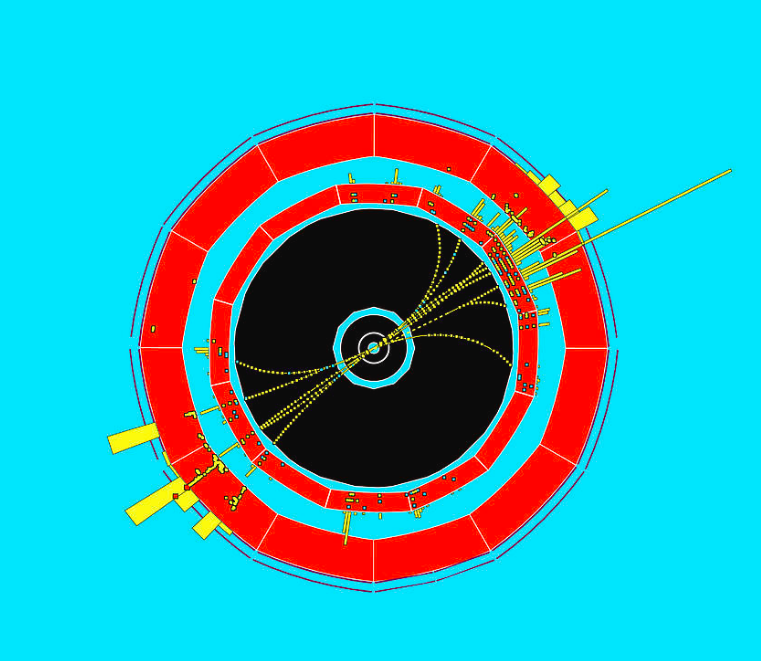
\includegraphics[width=0.50\textwidth]{Figures/Chapter1/DijetEvt.png}
\caption{The schematic display of a di-jet event from the ALEPH (a particle detector at the Large Electron-Positron collider) Experiment at the Large Electron-Positron Collider (LEP) is shown above. We can see two sprays of back to back particles within narrow cone, representing a di-jet event.}
\label{dijet}
\end{center}
\end{figure} 


Since we know QGP a color deconfined state of matter, an energetic parton carrying color charge traveling through the QGP medium is expected to lose a substantial a mount its energy to the medium. This is similar the effect that an electron beam losing energy in the electron-ion plasma via electromagnetic interaction \cite{ELossPlasma}. We call this effect as jet quenching. Figure \ref{JetELoss} shows jet quenching in QGP in AA collisions compared to pp collisions

\begin{figure}[hbtp]
\begin{center}
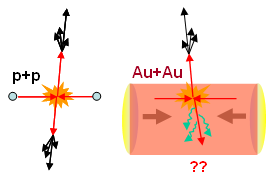
\includegraphics[width=0.45\textwidth]{Figures/Chapter1/JetELoss.png}
\caption{The schematic picture explaining jet quenching is shown above. Hard scatterings in pp collisions produce back-to-back "jets" of particles, but in Au + Au collisions, the presence QGP modifies the jets' properties.}
\label{JetELoss}
\end{center}
\end{figure} 


Experimentally, compared to pp collision where the QGP is not expected to be created, the jet spectra is modified by the QGP medium. The angular distributions would be broaden due to interaction with the medium. The $p_T$ spectra will be shifted to the left due to energy loss. This can be quantified by jet nuclear modification factor $R_{AA}$ similar to the $R_AA$ for quarkonium suppression mentioned previously. Figure \ref{JetRAA} shows the hadron angular correlation with the STAR experiment at RHIC and jet $R_{AA}$ as a function of $p_T$ with the ALICE experiments at LHC \cite{STARJetRef,ALICEJetRef}:
  
\begin{figure}[hbtp]
\begin{center}
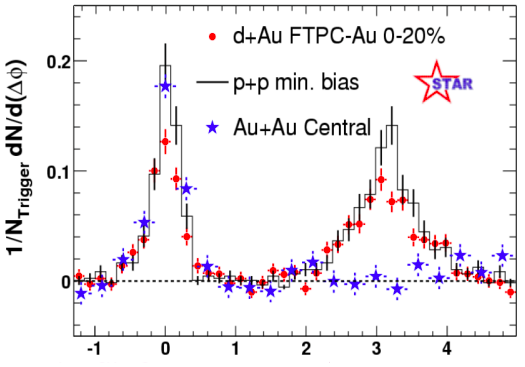
\includegraphics[width=0.55\textwidth]{Figures/Chapter1/HadronAngularSTAR.png}
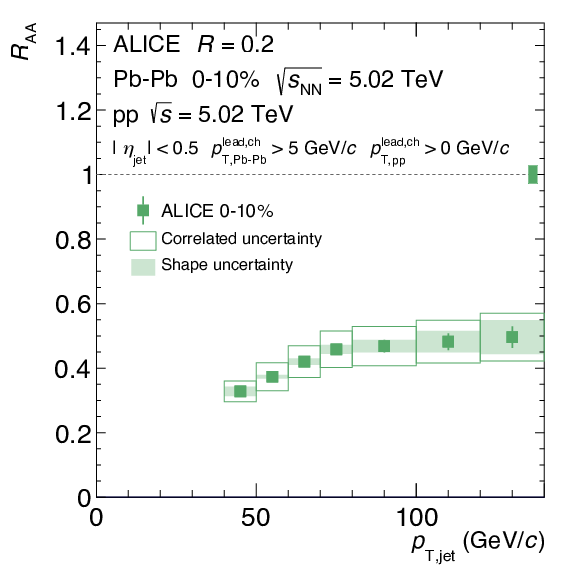
\includegraphics[width=0.40\textwidth]{Figures/Chapter1/JetRAAALICE.png}
\caption{The comparison of two-particle azimuthal distributions for central d + Au collisions to those seen in $pp$ and central Au + Au collisions measured with the STAR experiment and the jet $R_{AA}$ as a function $p_T$ measured by the ALICE experiment at LHC (right). From the STAR result, in central Au + Au collisions, the back-to-back peak has disappeared due to the redistribution of jet energy to the slow expanding medium constituents. The jet $R_{AA}$ from ALICE measurement is clearly below 1, suggesting that jets lose significant fractions of energy in $AA$ collision compared to $pp$.}
\label{JetRAA}
\end{center}
\end{figure} 

The jet $R_{AA}$ are all below 1 at RHIC and LHC \cite{ALICEJetRef,CMSJetSub}, which suggests jet quenching in AA collisions, supporting existence of QGP.

\subsection{Elliptic Flow} 

The reaction region in heavy-ion collisions, where the two nuclei overlap with each other, has an almond shape, which is azimuthally asymmetric. If the color deconfined matter QGP is created, particles emitted from the almond shape fire ball are expected to be azimuthally anisotropic due to differences of the pressure gradient of the QGP in the and their path length through QGP in the $x$ and $y$ directions. Experimentally, physicists Dr. Arthur Poskanzer (who sadly just passed away on June 30 2021) and Dr. Sergey Voloshin developed the event plane method to analyze the azimuthal anisotropy of particle emission in heavy-ion collisions \cite{EllipticFlow}. The reaction plane is defined as the plane of the impact parameter and the $x$-axis. Figure \ref{EventPlane} schematically shows the definition of reaction plane in heavy-ion collisions.

\begin{figure}[hbtp]
\begin{center}
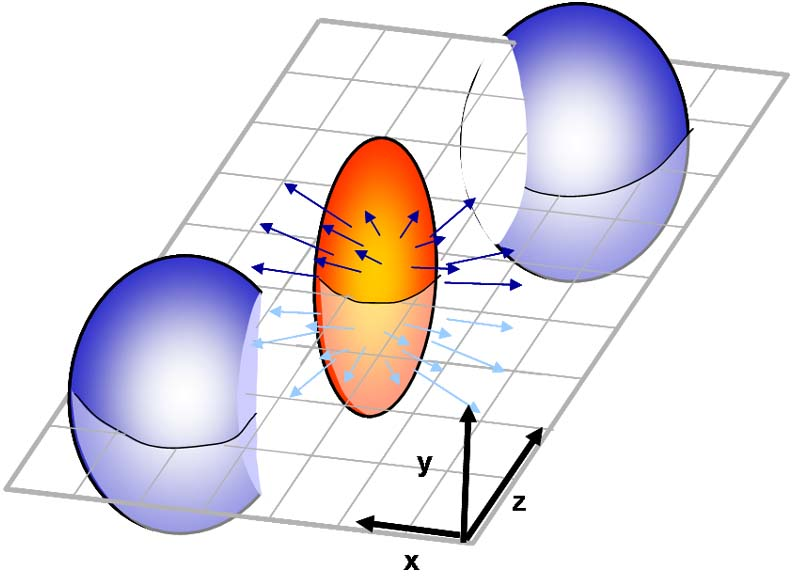
\includegraphics[width=0.40\textwidth]{Figures/Chapter1/ReactionPlane.jpg}
\caption{The figure above shows the ellipsoid of the overlapping nuclear reaction region of two nuclei in heavy-ion collisions. The reaction plane, which is the $x$-$z$ plane shown above, is constructed by the beam direction and the impact parameter vector. The emissions of particles are azimuthally anisotropic in the $x$-$y$ plane due to the geometry.}
\label{EventPlane}
\end{center}
\end{figure} 

The particle spectra in heavy-ion collisions can be factorized as 

\begin{equation}
E \frac{d^3N}{d^3p} = E \frac{1}{2 \pi p_T}\frac{d^3N}{dp_T dy d\phi} = E \frac{1}{2 \pi p_T} \frac{d^2N_1}{dp_T dy} \frac{dN_2}{d\phi}
\end{equation}

Since the particle emission is azimuthally anisotropic, we can expand the $F(p_T,\phi,y) = \frac{dN_2}{d\phi}$ into a Fourier series \cite{EllipticFlow}:


\begin{equation}
F(p_T,\phi,y) = \frac{x_0(p_T,y)}{2\pi}  + \sum_{n=1}^{\infty}[x_n(p_T,y)\cos(n\phi)+y_n(p_T,y)\sin(n\phi)] 
\end{equation}

According to trigonometry, we get

\begin{equation}
F(p_T,\phi,y)  = \frac{x_0(p_T,y)}{2\pi} + \sum_{n=1}^{\infty}2v_n(p_T,y)\cos[n(\phi - \Psi_{n})]
\end{equation}

Here, $v_n = \frac{1}{2} \sqrt{x_n^2 + y_n^2}$ and $\Psi_{n} =\frac{1}{n} \arctan(\frac{y_n}{x_n})$. 

To find the Fourier coefficients $v_n$, we can apply the Fourier tricks to find $x_n$ and $y_n$.


Theoretically, because the function $\frac{dN_2(\phi)}{d\phi}$ is continuously analytical, we can use integral to find the Fourier coefficients [18] 
\begin{equation}
x_n =2\int_{0}^{2\pi} \frac{dN_2(\phi)}{d\phi}\cos(n\phi)d\phi 
\end{equation}
\begin{equation}
y_n =2\int_{0}^{2\pi} \frac{dN_2(\phi)}{d\phi}\sin(n\phi)d\phi 
\end{equation}

Experimentally, because our data take on discrete values, we can convert the integral into a sum 
\begin{equation}
x_n =\frac{2}{N}\sum_{i=1}^{N} \cos(n\phi^i) = 2\langle \cos n\phi \rangle
\end{equation}
\begin{equation}
y_n =\frac{2}{N}\sum_{i=1}^{N} \sin(n\phi^i) = 2\langle \sin n\phi \rangle
\end{equation}

Here, we sum up all tracks in the experiment to get the $x_n$ and $y_n$. Then, we will be able to find 

\begin{equation}
v_n = \frac{1}{2} \sqrt{x_n^2 + y_n^2} = \sqrt{(\langle \cos n\phi \rangle)^2+(\langle \sin n\phi \rangle)^2}. 
\end{equation}




In heavy-ion physics, the first order Fourier coefficient $v_1$ is called the directed flow. 

\begin{equation}
v_1 =  \sqrt{(\langle \cos \phi \rangle)^2+(\langle \sin \phi \rangle)^2}. 
\end{equation}

It can be connected to the initial tilting source of the colliding nuclei \cite{V1Tilted} and can be used to study Chiral Magnetic Effect \cite{V1CME}. 

The second order Fourier coefficient $v_2$ is called elliptic flow. 

\begin{equation}
v_2 =  \sqrt{(\langle \cos 2\phi \rangle)^2+(\langle \sin 2\phi \rangle)^2} =  \sqrt{(\langle \cos^2 \phi \rangle - \langle \sin^2 \phi \rangle)^2 + (2  \langle \sin \phi \rangle \langle \cos \phi \rangle)^2}. 
\end{equation}

Assuming in initial stage before the collision, the sum of the momentum of two colliding nuclei $\vec p_1$ and $\vec p_2$ is exactly 0 without any fluctuation. That is

\begin{equation}
\vec{p_1} + \vec{p_2} = 0
\end{equation}

According to momentum conservation, for the final state particles, we have 

\begin{equation}
\sum_i^N p_x^i = 0
\end{equation}

\begin{equation}
\sum_i^N p_y^i = 0
\end{equation}

Therefore, we have

\begin{equation}
\langle p_T \cos \phi \rangle = \langle p_x \rangle = \frac{1}{N} \sum_i^N p_x^i   = 0
\end{equation}

\begin{equation}
\langle p_T \sin \phi \rangle = \langle p_y \rangle =  \frac{1}{N} \sum_i^N p_y^i  = 0
\end{equation}
 
But since the $p_T$ and $\phi$ are completely orthogonal, the random variable $p_T$ is uncorrected to $\phi$. Therefore, we have 
 
\begin{equation}
\langle p_T \cos \phi \rangle =  \langle p_T \rangle \langle  \cos \phi \rangle = 0
\end{equation}

\begin{equation}
\langle p_T \sin \phi \rangle =  \langle p_T \rangle \langle  \sin \phi \rangle = 0
\end{equation}

Finally, we know that $p_T > 0$, thus   
 
\begin{equation}
\langle p_T \rangle > 0
\end{equation}  
 
Hence,  


\begin{equation}
\langle \cos \phi \rangle =  0
\end{equation} 


\begin{equation}
\langle \sin \phi \rangle =  0
\end{equation}

Therefore, we have 

\begin{equation}
v_2 = \sqrt{(\langle \cos^2 \phi \rangle - \langle \sin^2 \phi \rangle)^2 + (2  \langle \sin \phi \rangle \langle \cos \phi \rangle)^2} = \langle \cos^2 \phi \rangle - \langle \sin^2 \phi \rangle. 
\end{equation}

In terms of momentum $p_x$ and $p_y$, we can rewrite $v_2$ as 

\begin{equation}
v_2 =  \langle \cos^2 \phi \rangle - \langle \sin^2 \phi \rangle = \langle\frac{p_x^2}{p_T^2} \rangle - \langle \frac{p_y^2}{p_T^2} \rangle = \langle \frac{p_x^2 - p_y^2}{p_T^2} \rangle = \langle \frac{p_x^2 - p_y^2}{p_x^2 + p_y^2} \rangle. 
\end{equation}

Classically, we know that the momentum is proportional to the pressure gradient. Schematically, we could write

\begin{equation}
p_x \simeq \frac{m\tau}{\rho}\frac{\partial P}{\partial x} \simeq \frac{m\tau}{\rho}\frac{P}{L_x}
\end{equation}

Where $m$ is the mass of the particle, $\tau$ is the life time of the QGP, $\rho$ is the density of the QGP, and $L_x$ is the minor axis of the ellipse in the x direction according to the geometry of Figure \ref{EventPlane}.

Likewise, we have the same relation for $p_y$

\begin{equation}
p_y \simeq \frac{m\tau}{\rho}\frac{\partial P}{\partial y} \simeq \frac{m\tau}{\rho}\frac{ P}{L_y}
\end{equation} 

Here,  $L_y$ is the major axis of the ellipse in the y direction according to the geometry of Figure \ref{EventPlane}. Apparently, $L_y > L_x$. 

Hence, we can write $v_2$ as 
\begin{equation}
v_2 =  \langle \frac{p_x^2 - p_y^2}{p_x^2 + p_y^2} \rangle = \frac{\frac{1}{L_x^2} - \frac{1}{L_y^2}}{\frac{1}{L_x^2} + \frac{1}{L_y^2}} =  \frac{L_y^2 - L_x^2}{L_x^2 + L_y^2}  > 0
\end{equation}

In heavy ion collision, we define the eccentricity $\epsilon_s$ of an ellipse is defined as \cite{V2Eccent}

\begin{equation}
\epsilon_s \equiv \frac{L_y^2 - L_x^2}{L_x^2 + L_y^2}
\end{equation}

Hence, we have

\begin{equation}
v_2 \simeq \epsilon_s
\end{equation}

Therefore, we can see that $v_2$ is essentially proportional to the eccentricity simply based on ellipse geometry of reaction region. Historically, $v_2$ has extensively studied experimentally and theoretically. It turns out light hadrons demonstrate collectivity. Their elliptic flow $v_2$ could be calculated using relativistic viscous hydrodynamics \cite{4DHydro}. If QGP is created, we expect $v_2$ of the light flavor hadrons to be positive as we derive above. Figure \ref{V2} show the $v_2$ as a function of $p_T$ of charged light flavor hadrons in heavy-ion collisions at mid-rapidity measured by RHIC and LHC experiment \cite{V2STAR,V2ALICE}

\begin{figure}[hbtp]
\begin{center}
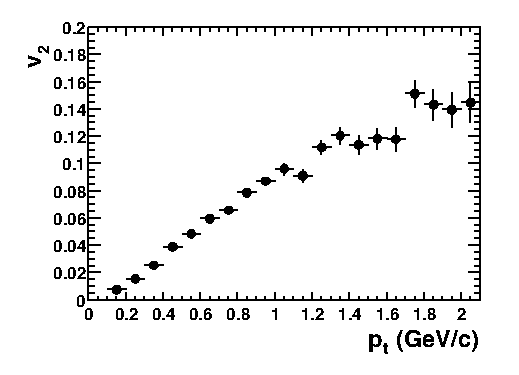
\includegraphics[width=0.45\textwidth]{Figures/Chapter1/STARV2Plot.eps}
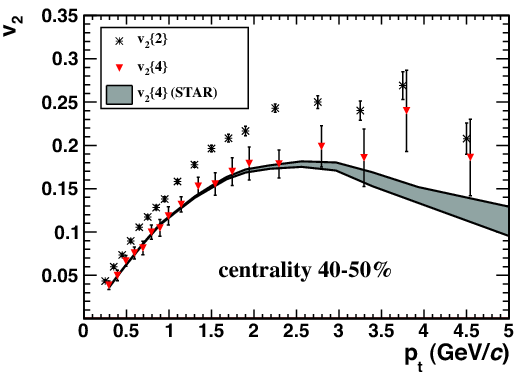
\includegraphics[width=0.45\textwidth]{Figures/Chapter1/ALICEV2Plot.png}
\caption{The elliptic flow $v_2$ of charged particles as a function of $p_T$ in Au + Au collision measured by the STAR experiments at RHIC (left) and in PbPb collisions by the ALICE experiments at LHC (right) are shown above. Clearly, $v_2 > 0$ is observed in both experiments.}
\label{V2}
\end{center}
\end{figure}   

We can clearly see positive $v_2$ of charged particles at both RHIC and LHC, which also supports the creation of QGP in high energy heavy-ion collisions.  
 
\subsection{Strangeness Enhancement} 

As described in Section 1.4.6, the temperature of QGP is well above 100 MeV, which is much larger than the strange quark mass (about 95 MeV). Therefore, since $T_{QGP} > m_s$, in the thermally and chemically equilibrated QGP, strange quarks could be produced thermally via the pair production processes: $u \bar u \rightarrow s\bar s$$, d \bar d \rightarrow s\bar s$, and $gg \rightarrow s \bar s$, establishing the chemical abundance equilibrium \cite{SSEnhance}. Therefore, the strangeness content in the QGP is enhanced, which could be experimentally observed from enhancement of strange particle yields in $AA$ collisions compared to $pp$ collisions. A direct experimental observable is the ratio of strange hadron yield to pions in $AA$ and $pp$ collisions scaled by $N_{part}$. Figure \ref{PhiRAA1} and \ref{PhiRAA2} show the measurements on strange mesons and baryons to pion ratios in $AA$ and $pp$ collisions at RHIC \cite{StrangeSTAR} and LHC \cite{StrangeALICE} 

\begin{figure}[hbtp]
\begin{center}
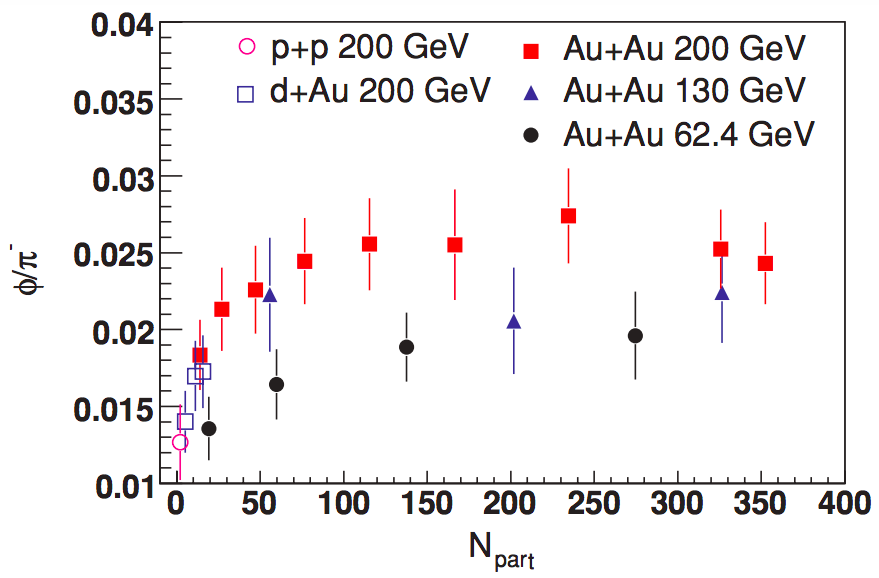
\includegraphics[width=0.50\textwidth]{Figures/Chapter1/STARPhiOverPi.png}
\caption{The yield ratio of $\phi/\pi$ as a function $N_{part}$ in $p + p$, $p + Au$, and $Au + Au$ from the STAR experiment at RHIC are shown above.}
\label{PhiRAA1}
\end{center}
\end{figure}   

\begin{figure}[hbtp]
\begin{center}
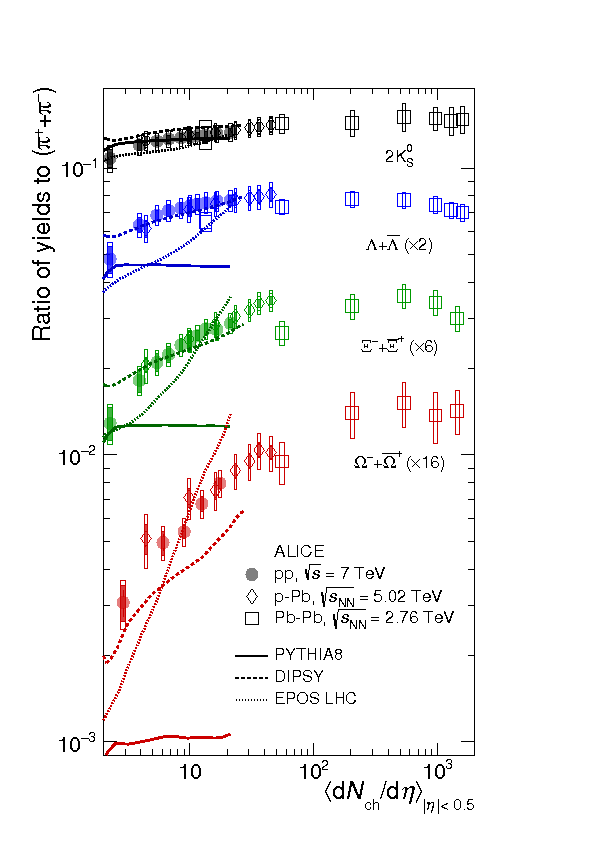
\includegraphics[width=0.60\textwidth]{Figures/Chapter1/ALICEStrange.png}
\caption{The yield ratio of strange hadrons $K^0_s, \Lambda^+, \Xi^0, \Omega^-$ as a function of $\langle dN_{ch}/d\eta \rangle$ from the ALICE experiment at LHC are shown above.}
\label{PhiRAA2}
\end{center}
\end{figure}   

We can see that $\phi/\pi$ ratio increases as $N_{part}$ and $\sqrt {s_{NN}}$ increases, which indicates strangeness enhancement in $AA$ collisions compared to $pp$ collisions. This again could be served as an evidence for the formation of QGP in heavy-ion collisions at RHIC and LHC. 

%J/psi suppression, jet quenching, elliptic flow, strangeness enhancement 

\subsection{Macroscopic Properties}

Physicists have conducted extensive studies to understand macroscopic properties of QGP. Below are some of the interesting properties of QGP observed in experiments:

\textbf{Transient Lifetime:} According to the experimental results at RHIC and LHC, QGP has a very short lifetime. It is on the order of 10 fm/c \cite{QGPLifeTime}. It is generally assumed that QGP reaches thermal \cite{QGPThermal} and near chemical equilibrium \cite{QGPChemical} via the strong interaction. So far, there is not sufficient experimental evidences to directly support this assumption.

\textbf{Strong Interacting System:} Moreover, QGP, as a deconfined state of matter, demonstrates a strongly interacting behavior, which contradicts to the prediction weak coupling according to the asymptotic freedom of quarks and gluons in QCD \cite{QCDAsym}. At $T \sim 1 - 3$ $T_c$, the coupling strength of QGP is still strong: $g_s \sim O(1)$ \cite{sQGP}. Therefore, strong interaction between the QGP constituents is in general non-perturbative. The equation of state of strong interacting QGP, as an input for hydrodynamic calculations, can be calculated by models such as MIT Bag Model \cite{MITBag} or Lattice QCD \cite{LatticeEOS}. 

\textbf{Perfect Liquid Behavior:} Finally, QGP demonstrates nearly perfect liquid properties. The expansion of QGP in the fireball stage is approximately isentropic and could be well described by hydrodynamics \cite{Bjorken}. More specially, due to the relativistic nature of the strongly coupled near-perfect liquid system, assuming QGP reaches thermal \cite{QGPThermal} and near chemical equilibrium \cite{QGPChemical}, relativistic viscous hydrodynamics \cite{4DHydro} is the correct theoretical formalism to describe the dynamics of QGP. As an nearly perfect liquid, the shear viscosity to entropy density ratio of the QGP is very small: $\frac{\eta}{s}\sim (1 - 2.5) \frac{1}{4\pi}$ \cite{QGPEtaOverS}, approaching the quantum limit $\frac{\eta}{s} = \frac{1}{4\pi}$ predicted by the strongly coupled $N=$4 supersymmetric Yang-Mills plasma in Anti-de-Sitter Space/Conform Field Theory (AdS/CFT) correspondence \cite{ADSCFT}.

\textbf{Color Opaque Plasma:} It is also interesting that QGP is a color opaque plasma \cite{QGPGen}. This means that gluons propagating through the QGP will be absorbed by the plasma medium. Experimentally, the suppression of hadrons is a measure of the color opacity of the QGP \cite{QGPGen}. Physicists have found that QGP is indeed highly color opaque \cite{QGPOpaque}.


%Nuclear Physics is a study of the interaction of nucleons and structure of atomic nuclei. 
%\subsection{Microscopic Structure}

%Constituents 

%Microscopic Kinetics -- Transport properties
 


\subsection{Open Questions}

However, although extensive studies have been carried out for many years, there are still many open questions, most of which are derived from the mysterious macroscopic behavior of QGP. Below is the list of selected open questions that are currently under active investigation by the heavy-ion physics community \cite{BigQuestions}:

1) \textbf{Thermalization of QGP:} How can QGP reach thermal equilibrium within such a short time, which is on the order 1 $fm/c$, from the non-equilibrium stage?

2) \textbf{Inner Workings of QGP:} What is the correct degree of freedom to describe the QGP? The inner workings of QGP, as a deconfined phase of matter, must lay between asymptotically free quarks and gluons and color neutral hadrons. That is also why the sPHENIX experiment at RHIC, as the next generation DOE flagship Heavy Ion Physics program in the U.S., is going to built at BNL and collect date to probe the inner workings of QGP by resolving its properties at shorter and shorter length scales. 

3) \textbf{Smallest Droplet of QGP:} What is the smallest droplet of QGP that can be created? Can QGP be created in pPb, $pp$, or even $e^+e^-$ collision systems? What are the limits of the applicability of hydrodynamics?

\section{Heavy Flavor Physics}


\subsection{Open Heavy Flavor Physics}

My graduate research focuses on answering the second question through the data analysis of fully reconstructed heavy flavor hadrons with the CMS experiment to understand transport properties and probe the microscopic structure of QGP. In this section, we will focus on discussing open heavy flavor physics where the only one heavy quark $Q$ is in hadron. Open heavy flavor hadrons have $\pm 1$ heavy flavor number. Quarkonia states $Q\bar Q$ are considered as hidden heavy flavor with a zero net heavy flavor quantum number. Their properties are very different from open heavy flavor hadrons. We will not discuss them in this thesis and focus only on open heavy flavor physics. 

\subsection{Heavy Quarks}

Heavy quarks, such as charm and beauty quarks, whose masses are on the order of GeV, lie in a scale above both $\Lambda_{QCD}$ and $T_{QGP}$. Therefore, they are predominantly produced in the early stage of heavy-ion collisions where hard scattering processes occur. Their production could be calculated by perturbation QCD. Figure \ref{HQProduce} shows the lowest order Feynman diagrams of heavy quark pair production in QCD. 

 \begin{figure}[hbtp]
\begin{center}
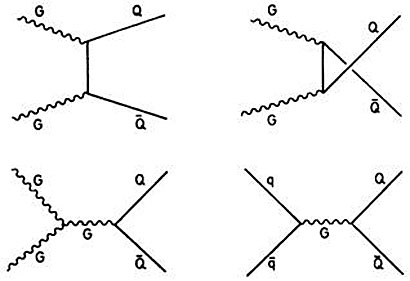
\includegraphics[width=0.45\textwidth]{Figures/Chapter1/HQDiagram.jpg}
\caption{The four lowest order tree level Feynman diagrams of heavy quark pair production are shown above.}
\label{HQProduce}
\end{center}
\end{figure}   

In general, due to their relatively small momentum transfer to the QGP medium constituents compared to their large masses \cite{HQReview}, they should not reach complete thermalization via multiple scattering as they traverse through the QGP. In addition, since their lifetime is much longer than the QGP lifetime, they retain their identities and record the evolution of the QGP, which makes them excellent probes. Then, they travel through the medium, hadronize into heavy flavor hadrons, and decay weakly. Their decay product are detected and identified by particles detectors.

Experimentally, from the final stage decay products, we can fully reconstruct heavy flavor hadrons where the dynamics of heavy quarks is encoded with different transverse momenta to study their diffusion coefficients, hadronizaton mechanism, and energy loss to probe the microscopic structure of QGP via their scattering patterns with the QGP constituents at different wavelengths. Figure \ref{HQ} below shows respectfully an event of beauty quark production and hadronization in vacuum and QGP.

 \begin{figure}[hbtp]
\begin{center}
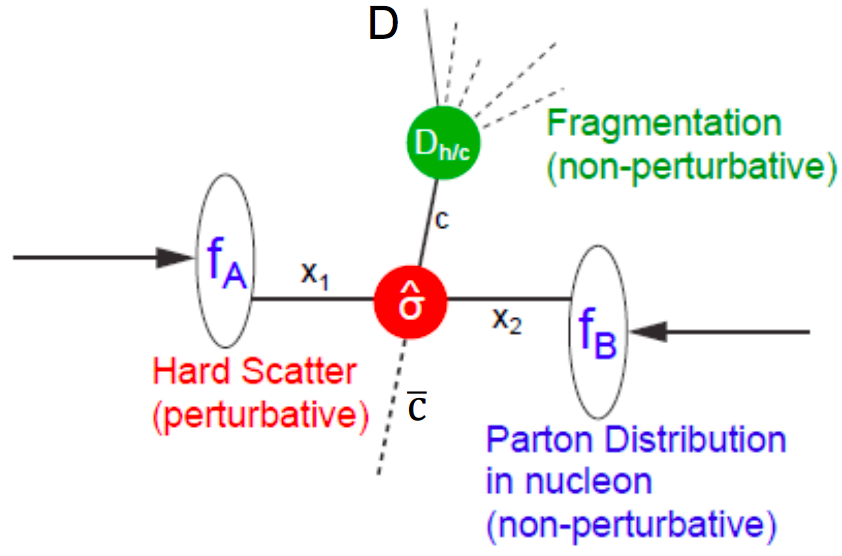
\includegraphics[width=0.46\textwidth]{Figures/Chapter1/HQVacuum.png}
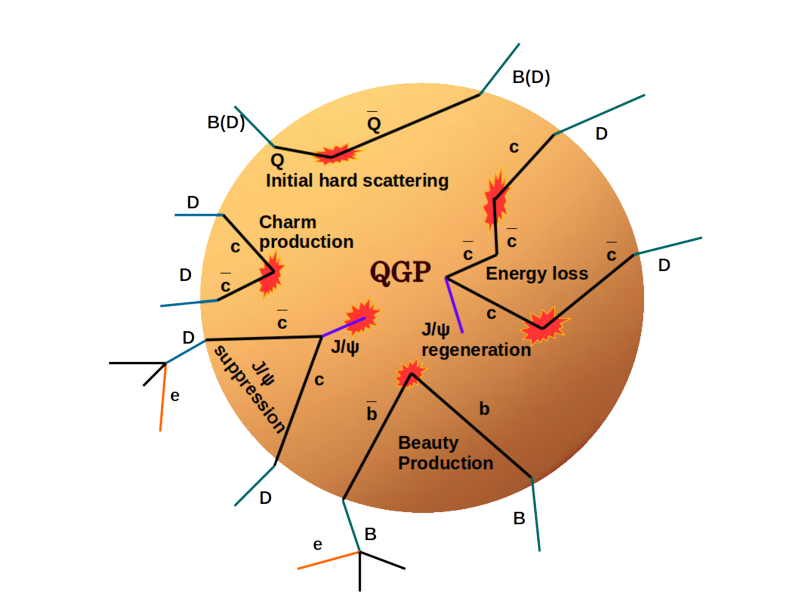
\includegraphics[width=0.48\textwidth]{Figures/Chapter1/HQQGP.png}
\caption{The schematic demonstrations of heavy quark production and hadronization in vacuum (left) and QGP (right) are shown above.}
\label{HQ}
\end{center}
\end{figure}   



\subsection{Heavy Flavor Physics in Vacuum}

To use heavy quark to probe the QGP created in heavy-ion collisions, we first need to understand heavy quark physics in vacuum from pp collisions. In the process $pp \rightarrow Q \bar Q$, QCD factorization theorem could be applied. High precision pQCD calculations, including next-to-leading order (NLO), Fixed-to-Next-to-the-Leading (FONLL) \cite{FONLLRef1,FONLLRef2}, A Variable-Flavour Number Scheme for NNLO (GM-VFNS) \cite{GM-VFNSRef}, and POWHEG \cite{POWHEGRef}, have been developed to describe heavy quark production. in $pp$ collisions Here, we will show FONLL calculations of charm and beauty quarks spectra, schematically denoted as: $\frac{d^2\sigma^Q}{p_T dp_T dy}$, in $pp \rightarrow Q  \bar Q$ at different energies \cite{FONLLCal}. Figure \ref{FONLL} shows the FONLL calculations of charm and beauty quarks spectra produced for $pp$ collisions at the LHC energy $\sqrt s = 5.02$ TeV.

 \begin{figure}[hbtp]
\begin{center}
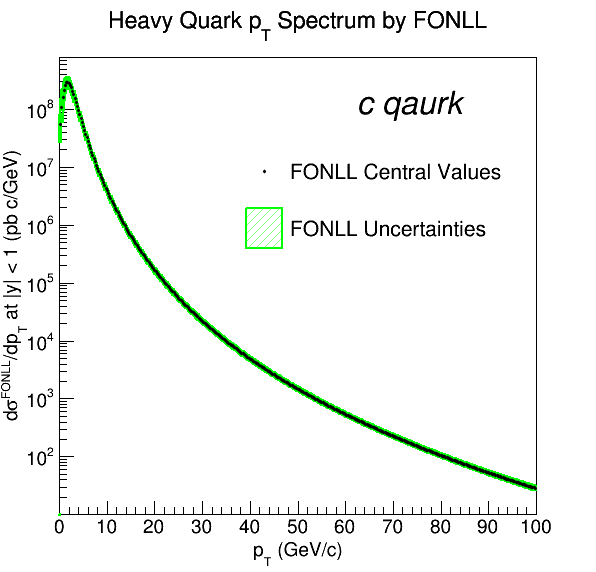
\includegraphics[width=0.48\textwidth]{Figures/Chapter1/Charm.png}
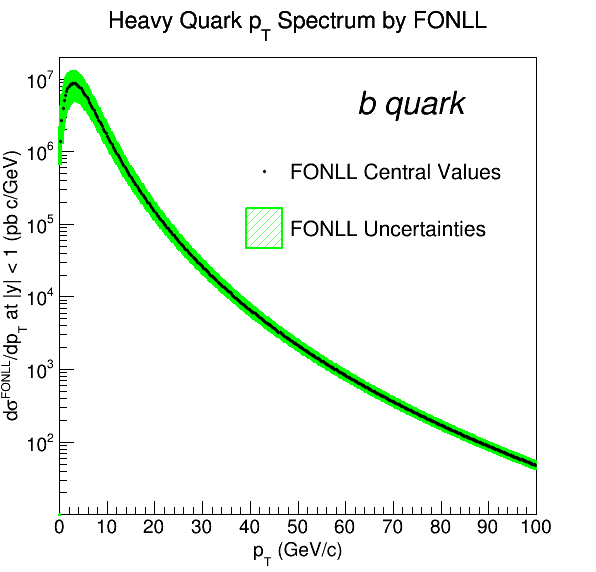
\includegraphics[width=0.48\textwidth]{Figures/Chapter1/Beauty.png}
\caption{The charm quark (left) and beauty quark (right) differential cross section $\frac{d\sigma}{dp_T}$ as a function transverse momentum $p_T$ at $|y| < 1$ from FONLL calculations, are shown above.}
\label{FONLL}
\end{center}
\end{figure}   

The comparison between different pQCD theoretical calculations and charm \cite{CMSD0RAA} and beauty \cite{CMSBPRAA} hadrons production in $pp$ collisions with the CMS experiment at the LHC is shown below in Figure \ref{pQCDppComp}   

 \begin{figure}[hbtp]
\begin{center}
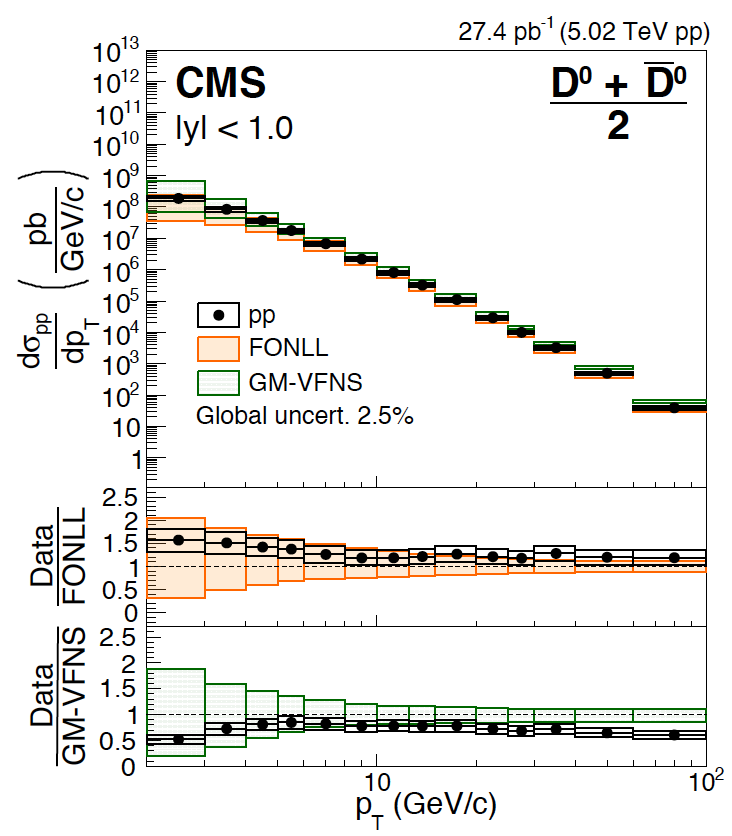
\includegraphics[width=0.48\textwidth]{Figures/Chapter1/pQCDppD0.png}
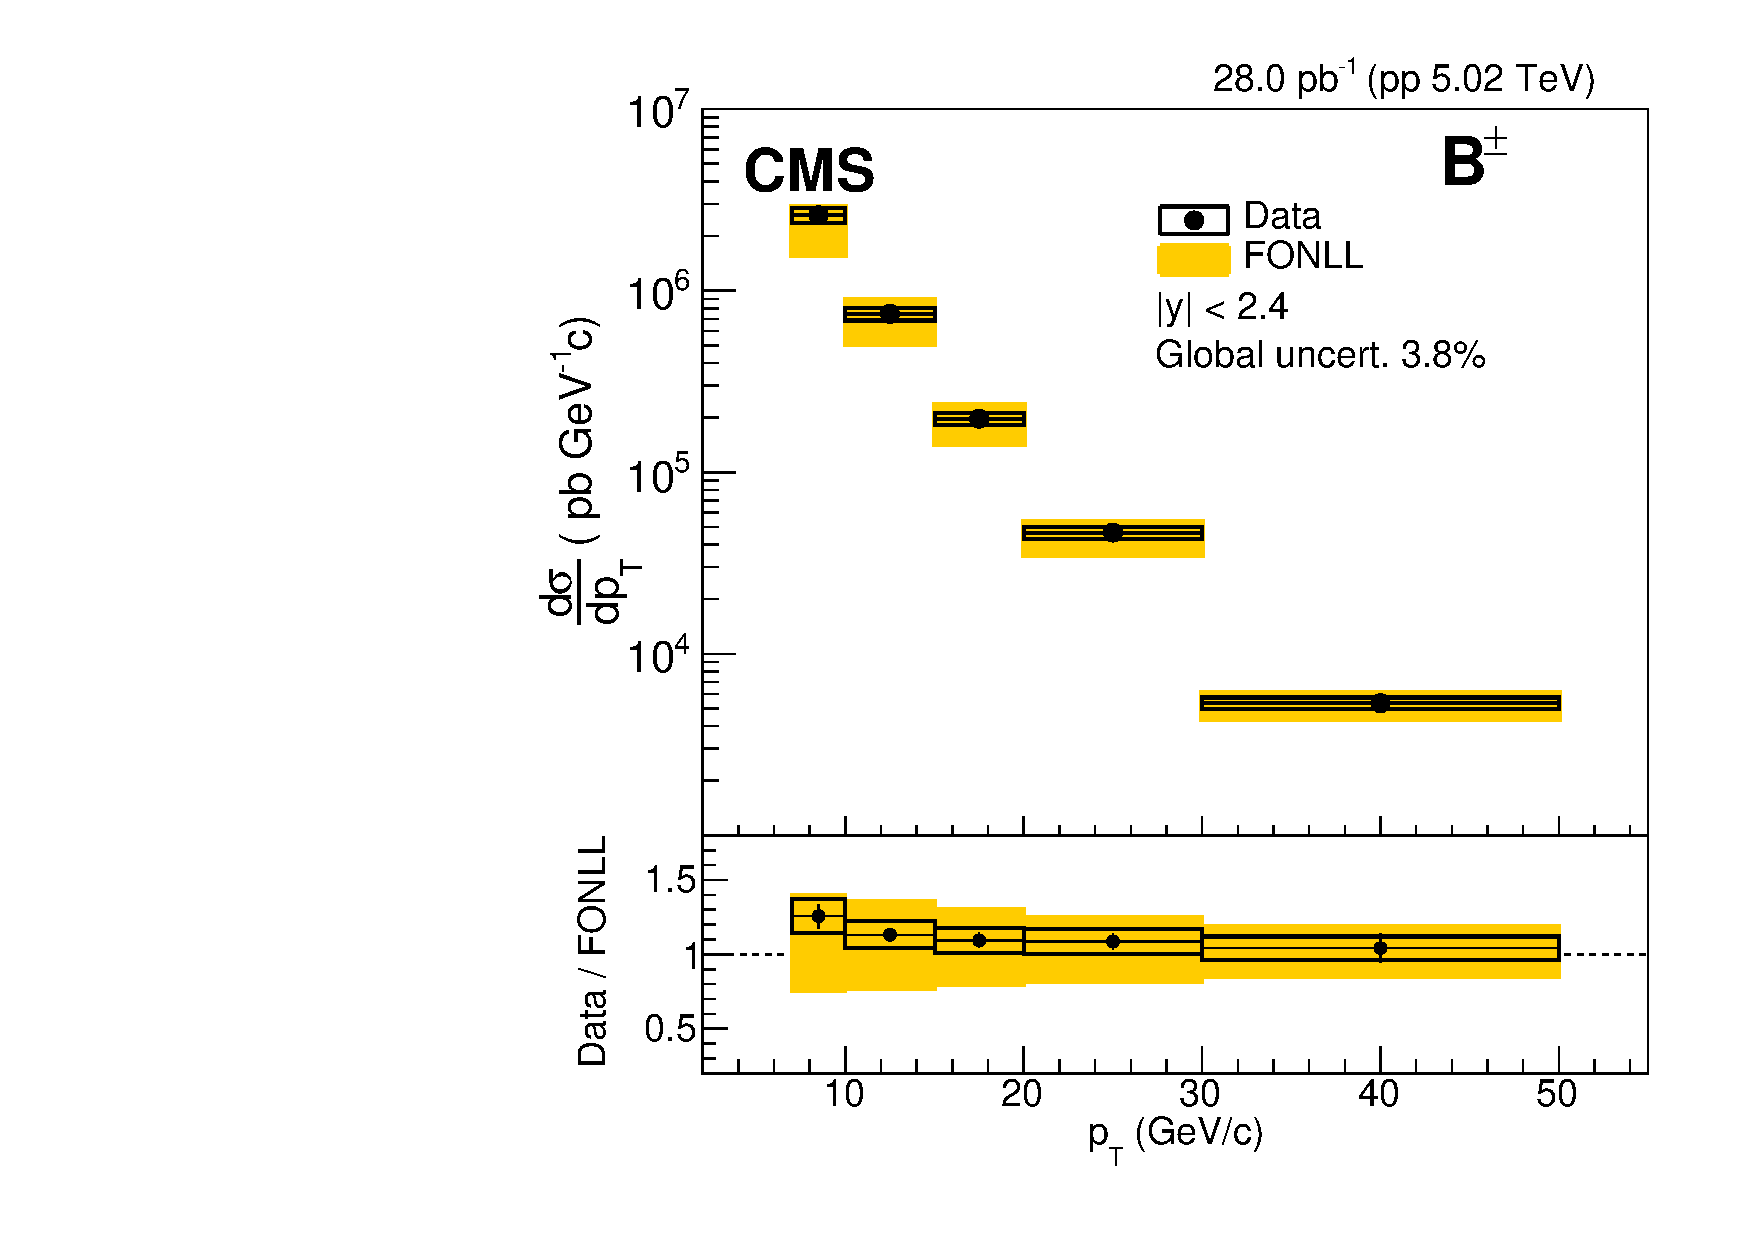
\includegraphics[width=0.48\textwidth]{Figures/Chapter1/pQCDppBP.pdf}
\caption{The charm quark (left) and beauty quark (right) $p_T$ spectra and the ratio with FONLL and GM-VFNS pQCD theoretical calculations are shown above.}
\label{pQCDppComp}
\end{center}
\end{figure}   

At higher $p_T$, reasonably good agreement between FONLL and GM-VFNS with the pp data for both $D^0$ and $B^+$ $p_T$ spectra. However, at lower $p_T$, FONLL tends to under predict the data while GM-VFNS tends to overshoot the data. Both of the calculation have large theoretical uncertainties at low $p_T$ as the applicability of pQCD starts breaking down in softer collisions. 
 
In vacuum, heavy quarks fragment into heavy flavor hadrons $Q \rightarrow H_Q$. We can defined the parton fragmentation function $D^{H_Q}_{i}(z,\mu^2)$ where is the probability for a quark $q$ with energy $E$ fragment into a hadron with energy $zE$ ($0 < z < 1$) at the factorization scale of $\mu^2$ \cite{QCDFFunc}. According to pQCD, $D^{H_Q}_{i}(z,\mu^2)$ is universal in vacuum from $e^+e^-$, $ep$, and $pp$ collisions. Figure \ref{FFProcess} shows the scattering processes which fragmentation fraction is involved:

 \begin{figure}[hbtp]
\begin{center}
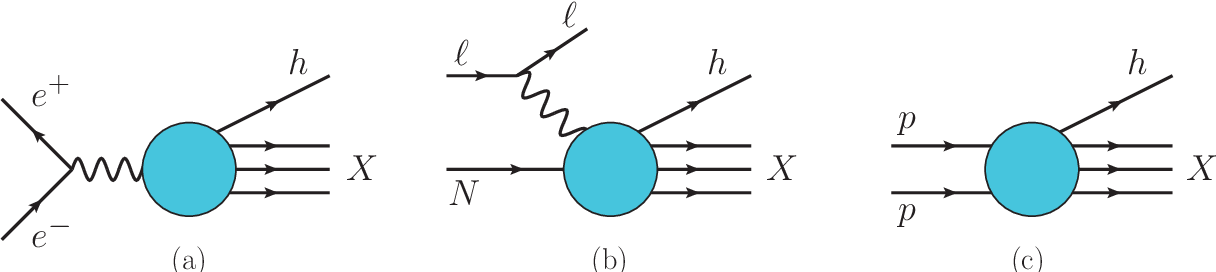
\includegraphics[width=1.0\textwidth]{Figures/Chapter1/FFProcess.png}
\caption{Single-inclusive hadron production process, where fragmentation function are involved, in (a) electron-positron annihilation, (b) deep-inelastic lepton-nucleon scattering, (c) proton-proton scattering are shown above.}
\label{FFProcess}
\end{center}
\end{figure}   

Next, we are ready to define heavy quark fragmentation fraction $f(Q \rightarrow H_Q)$. First we know, the energy

\begin{equation}
E=  \sqrt{m^2 + p_T^2 \cosh^2 y}
\end{equation}

Ignoring the mass, we have

\begin{equation}
E \simeq p_T \cosh y
\end{equation}

So energy of the hadron $E^h$ where the quark with $E^Q$ fragments into will be


\begin{equation}
E^h  = z E^Q 
\end{equation}

So we have the transverse momentum of the hadron $p_T^h$ 

\begin{equation}
p_T^{H_Q} = z p_T^Q
\end{equation}

With heavy quark spectra $ \frac{d^2\sigma^Q}{p_T dp_T dy}$ and parton fragmentation function $D_{i}^{H_Q}(z,\mu^2)$, we let


\begin{equation}
 \frac{d^2\sigma^Q}{p_T dp_T dy} = F^Q(p_T, y)
\end{equation}


Hence, for a hadron with $p_T$, the heavy quark will have $p_T/z$ with probability $D^{H_Q}_{i}(z)$ to fragment into this hadron. Therefore, the heavy flavor hadron spectra is given by:

\begin{equation}
\frac{d^2\sigma^{H_Q}}{p_T dp_T dy} = \int_{x_T}^1 F^Q(p_T/z, y) D_{i}^{H_Q}(z,\mu^2) dz
\end{equation}

Here $x_T = \frac{2p_T}{\sqrt s}$ \cite{HadronScale}.







\iffalse



From Figure \ref{FONLL} , it looks like the $p_T$ spectra of heavy quarks is overall approximately power law, particularly at high $p_T$. In fact, at a fixed $x_T$ and the center of mass angle \cite{HadronScale}, the heavy quark spectra overall demonstrates the power like behavior. In addition, assuming the spectra $F^Q(p_T,y)$ factorizes, we have
 

\begin{equation}
F^Q(p_T, y) \sim g(y) p_T^{-n}
\end{equation}

Hence,

\begin{equation}
F^Q(p_T/z, y) \sim F^Q(p_T, y)/z^{-n} = F^Q(p_T, y) z^n
\end{equation}


\begin{equation}
\frac{d^2\sigma^{H_Q}}{p_T dp_Tdy} \simeq \int_{x_T}^1 F^Q(p_T, y)  z^{n} D^{H_Q}_{i}(z) \frac{dz}{z^2} =F^Q(p_T, y)  \int_{x_T}^1  z^{n-2} D^{H_Q}_{i}(z) dz
\end{equation}



Hence, we can define the approximately constant heavy quark fragmentation fraction $f_{Q \rightarrow H_Q}$ as follows

\begin{equation}
f(Q \rightarrow H_Q) = \int_{x_T}^1 z^{n-2} D^{H_Q}_{i}(z) dz
\end{equation}

Hence, we will get 

\begin{equation}
\frac{d^2\sigma^{H_Q}}{p_T dp_T dy} = f(Q \rightarrow H_Q)  \frac{d^2\sigma^Q}{p_T dp_T dy}
\end{equation}

\fi

Now if we consider a factorization scale near the heavy quark mass $\mu^2 \rightarrow m_Q^2$, according to PDG reference \cite{AlphaTheoEx}, solving the leading evolution equation, the heavy quark fragmentation function $D_Q^{H_Q}(z)$ is in a form of delta function and light quark $q$ and gluons $g$ ($i = g, q$) will not contribute to produce heavy flavor hadrons. Hence, we could write

\begin{equation}
D^{H_Q}_{q,g}(z,\mu^2)|_{\mu^2=m_Q^2} = 0
\end{equation}

In fact, the Peterson Fragmentation Function of heavy quarks $D^{H_Q}_Q(z,\epsilon_Q)$ is given by \cite{Peterson}

\begin{equation}
D^{H_Q}_Q(z,\epsilon_Q) = \frac{N}{z[1-1/z-\epsilon_Q/(1-z)]^2}
\end{equation}

Here, $N$ is the normalization constant such that $\int_0^1 D^{H_Q}_Q(z,\epsilon_Q) dz = 1$. $\epsilon_c = $ 0.03 and $\epsilon_b = $0.005. The comparison between the Peterson fragmentation function of beauty quarks and the delta function is shown below

\begin{figure}[hbtp]
\begin{center}
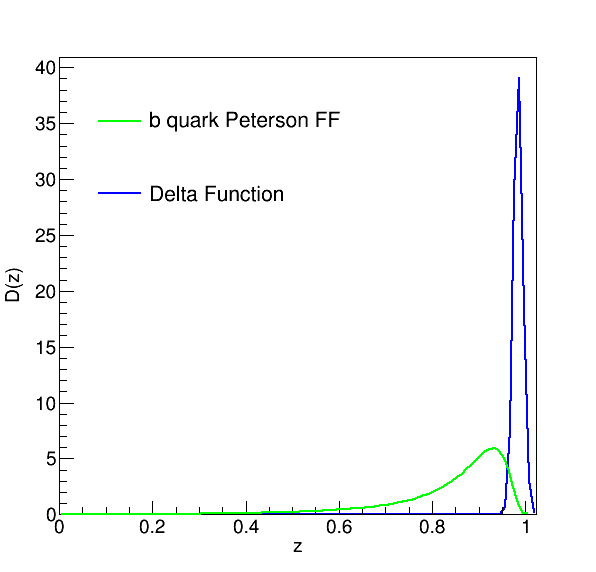
\includegraphics[width=0.65\textwidth]{Figures/Chapter1/FFPeterson.png}
\caption{The comparison between the Peterson fragmentation function (green) and the delta function (blue) is shown above.}
\label{FONLL}
\end{center}
\end{figure}   


Graphically, we find that the Peterson fragmentation function can be roughly approximated by delta function. In fact, when $\epsilon_Q = $0, the Peterson fragmentation function is essentially a delta function $D^{H_Q}_{Q}(z,\epsilon_Q = 0) \simeq \delta(1 - z)$. Hence, we can define

\begin{equation}
D^{H_Q}_{Q}(z,\mu^2)|_{\mu^2=m_Q^2} = f(Q \rightarrow H_Q) \delta(1 - z)
\end{equation}

Here $f({Q \rightarrow H_Q})$ is the heavy quark fragmentation fraction and stands for the probability of a heavy quark $Q$ hadronize into an open heavy flavor hadron $H_Q$. Indeed, according to the momentum sum rule that constrains the parton fragmentation function \cite{QCDFFunc}

\begin{equation}
\sum_{H_Q} \int_0^1 z D^{H_Q}_{Q}(z,\mu^2) dz = 1
\end{equation}

\begin{equation}
\sum_{H_Q} \int_0^1 z f(Q \rightarrow H_Q) \delta(1 - z) dz = 1
\end{equation}

\begin{equation}
\sum_{H_Q} f(Q \rightarrow H_Q) = 1 
\end{equation}

This verifies that the sum of heavy quark fragmentation fraction over all heavy flavor hadrons is equal to unity. Next, we have 


\begin{equation}
\frac{d^2\sigma^{H_Q}}{p_T dp_T dy} = \int_{x_T}^1 F^Q(p_T/z, y) D_{i}^{H_Q}(z,\mu^2) dz =  \int_{x_T}^1 F^Q(p_T/z, y) D^{H_Q}_{Q}(z,m_Q^2) dz 
\end{equation}

Thus,

\begin{equation}
\frac{d^2\sigma^{H_Q}}{p_T dp_T dy}  = \int_{x_T}^1 F^Q(p_T/z, y) f(Q \rightarrow H_Q) \delta(1 - z) dz =  f(Q \rightarrow H_Q)  F^Q(p_T, y)
\end{equation}

Hence, we have 

\begin{equation}
\frac{d^2\sigma^{H_Q}}{p_T dp_T dy} = f(Q \rightarrow H_Q) \frac{d^2\sigma^{Q}}{p_T dp_T dy}
\end{equation}

This means that the open heavy flavor hadron spectra $\frac{d^2\sigma^{H_Q}}{p_T dp_T dy}$ is essentially proportional to the heavy quark spectra $\frac{d^2\sigma^{Q}}{p_T dp_T dy}$ with heavy quark fragmentation fraction $f(Q \rightarrow H_Q)$ the as the coefficient of proportionality. Experimentally, charm and beauty fragmentation fractions have been measured at LEP, HERA, and the LHC and documented in PDG \cite{AlphaTheoEx}. The fragmentation fraction is often treated roughly a constant independent to $p_T$, $y$, and $\sqrt s$ and is assumed to be universal in $e^+e^-$, $ep$, and $pp$ collisions systems \cite{AlphaTheoEx}. 

In terms of being a constant, according LHCb $pp$ results \cite{LHCbFF}, it appears that the fragmentation fraction has significant $\sqrt s$ and $p_T$ dependence while no significant $y_B$ (or $\eta_B$) dependence is observed. Figure \ref{BeautyFFLHCb} shows the beauty quark fragmentation fraction: $f_u = f(b \rightarrow B^+)$, $f_d = f(b \rightarrow B^0)$, and $f_s = f(b \rightarrow B_s^0)$

 \begin{figure}[hbtp]
\begin{center}
\includegraphics[width=0.60\textwidth]{Figures/Chapter1/LHCbFFs.png}
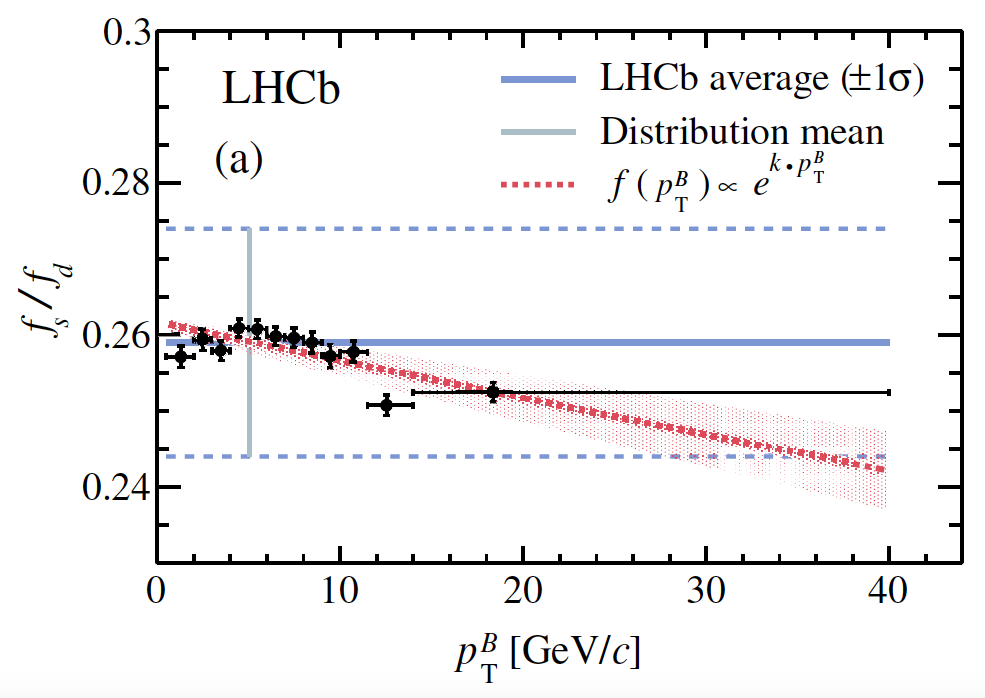
\includegraphics[width=0.60\textwidth]{Figures/Chapter1/LHCbFFpT.png}
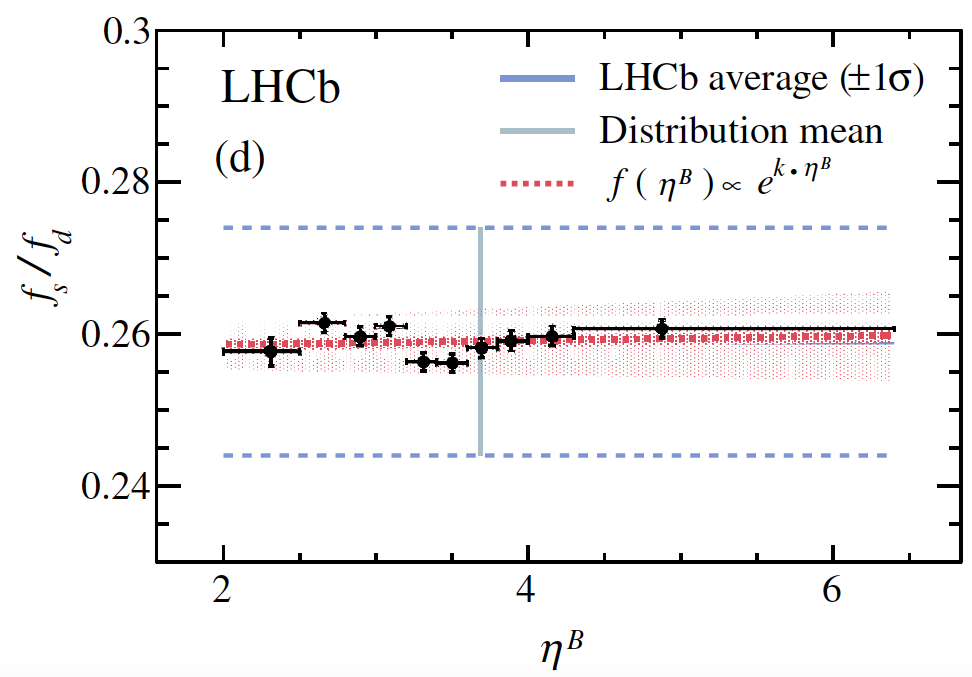
\includegraphics[width=0.60\textwidth]{Figures/Chapter1/LHCbFFy.png}
\caption{ $R$, the corrected yield ratio of $B^0_s/B^+$, as a function the $pp$ collision energy $\sqrt s$ (top), the $f_s/f_d$ ratio as a function $p_T$ (middle), and the $f_s/f_d$ ratio as a function $\eta_B$ (bottom), from the LHCb experiment are shown above.}
\label{BeautyFFLHCb}
\end{center}
\end{figure}   


In terms of universality, according to Strangeness Quark Matter Conference (SQM) in 2021, a hadronization universality breaking is observed from the ALICE experiment at the LHC \cite{GMISQM}. Figure \ref{CharmFFALICE} shows the hadronization universality breaking reported by the ALICE experiment in SQM 2021

 \begin{figure}[hbtp]
\begin{center}
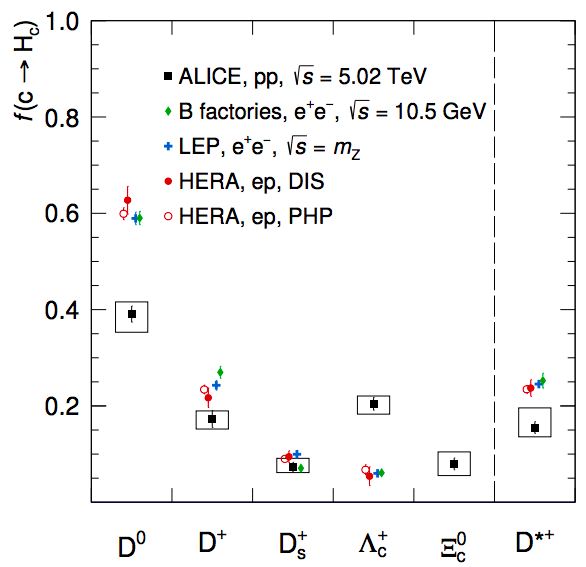
\includegraphics[width=0.52\textwidth]{Figures/Chapter1/ALICECharmFF.png}
\caption{The charm quark fragmentation fraction to different charm hadrons species in $e^+e^-$, $ep$, and $pp$ collisions are presented above. From the ALICE experiment, we can clearly see that the fragmentation fraction of $D^0$ has drop by about 40\% while the $\Lambda_c^+$ has enhanced by about a factor of 4. Therefore, the hadronization universality is clear broken at the LHC energy in the charm sector.}
\label{CharmFFALICE}
\end{center}
\end{figure}   

Further investigations of these results are currently ongoing. However, we will not expand the discussions here. Now, equipped with the understanding of heavy flavor physics in vacuum from $pp$ collisions as a reference, we are ready to use heavy quarks to study QGP created in heavy-ion collisions. 

\subsection{Heavy Quark Diffusion}

In the limit of low $p_T$ or equivalently long wavelength, for heavy quarks inside the QGP medium, the elastic collision cross section dominates. In elastic $Q q \rightarrow Q q$ process in the thermally equilibrated QGP medium, heavy quarks has the relatively small momentum transfers on the order of the temperature compared to the heavy quark mass: $m_Q > |k| \simeq T$. Considering the mean free time of HQ in the QGP medium is about $\tau \sim 0.44 fm/c$ \cite{HQTau}. Therefore, the number of scattering of heavy quarks in the QGP medium is about $n \sim \frac{\tau_{QGP}}{\tau_{HQ}} \simeq 23 \sim O(10)$.

Now, we can consider a simple binomial process to model the diffusion of heavy quark in the QGP medium. Assuming the momentum of the heavy quark at $t = 0$ is $p$, after the time $\tau_{HQ}$, one scattering happens. The momentum of the heavy quark at $t = \tau_{HQ}$ either $p + k$ or $p - k$. Each has $1/2$ probability. Next, after another $\tau_{HQ}$, another scattering happens. The momentum of the heavy quark at $t = 2\tau_{HQ}$ either $p + 2k$, $p$ or $p - 2k$ with $1/4$, $1/2$, and $1/2$ probability respectfully. Therefore, the standard deviation of binomial process $\sigma_p = \frac{\sqrt{n}}{2} k$. If we take $n = 25$, $\sigma_p = 2.5k \simeq 2.5 T_{QGP} =$ 0.4 GeV. Experimentally, we consider a heavy quark with momentum about $p  > $ 1.5 GeV/c $>> \sigma_p$. According to Figure \ref{FONLL}, we could see that the heavy quark transverse momentum is well above 1 GeV/c. Hence, such heavy quarks still retain a lot of memory about its initial conditions even after multiple small scattering with QGP medium. Hence, in these conditions, heavy quark undergoes Brownian-like motion in the QGP medium \cite{HQReview}. Their motion in the QGP medium could be characterized by the Planck-Fokker Equation, which could be schematically written as follows \cite{HQRaff}:

\begin{equation}
\frac{\partial}{\partial t} f_q(t, \vec{p}) = \frac{\partial}{\partial p_{i}} \{ A_i(\vec p) f_q(t,\vec{p}) + \frac{\partial}{\partial p_j}[B_{ij}(\vec{p})f_q(t,\vec{p}) ] \}
\end{equation}

Here, $f_q(t,\vec{p})$ is the heavy quark phase space distribution function. If we ignore the modification of the cold nuclear matter effects on the heavy quark initial production spectra, then in heavy-ion collision:

\begin{equation}
F^Q( t = 0,p_T) \propto \frac{d\sigma_{FONLL}}{p_Tdp_T}
\end{equation}

$A_i(\vec p)$ and $B_{ij}(\vec p)$ are transport parameters. 

\begin{equation}
A_i(\vec p) = A(\vec p) p_i
\end{equation}


The transport parameters $A_i(\vec{p})$ is related to the thermal relaxation rate and $B_{ij}(\vec{p})$ is related to the momentum diffusion of heavy quarks \cite{HQReview}. The heavy quark special diffusion coefficient $D_s$ is related to the transport parameter as follows:

\begin{equation}
D_s = \frac{T} {m_Q A(p=0)}
\end{equation}

$D_s$ characters the fundamental property of the QGP $\frac{\eta}{s}$ via the relationship 

\begin{equation}
2 \pi T D_s \simeq \frac{\eta}{s}
\end{equation}

More detailed studies have been carried out to examine heavy quark coupling strength and quantify the information heavy quarks carry as they traverse through the QGP medium \cite{HQJamie}.


\subsection{Heavy Quark Energy Loss}

In the limit of high $p_T$ or equivalently short wavelength, inelastic cross section starts to dominate \cite{HQReview}. Heavy quarks lose a substantial amount of energy as they travel fast through the QGP medium \cite{HQELossFirst}. In a simplified schematization, there are two different pictures that describe the energy loss mechanism of heavy quark in the QGP medium. In the pQCD picture, the coupling of the constituents of the QGP is assumed to be weak. Therefore, the QGP is made of weakly coupled quasiparticles. Heavy quarks scatter off the constituents incoherently when propagating through the QGP medium. There are two energy loss mechanisms: collisional energy loss and radiative energy loss \cite{HQRaff}. The collisional energy loss is given by $-\frac{dE}{dx} = \kappa_{coll}T^2$ and the radiative energy loss is given by  $-\frac{dE}{dx} = \kappa_{rad}T^3x$ \cite{HQCollELoss,HQRadELoss}. Figure \ref{HQELosspQCD} shows schematically heavy quark energy loss mechanism in the QGP medium



 \begin{figure}[hbtp]
\begin{center}
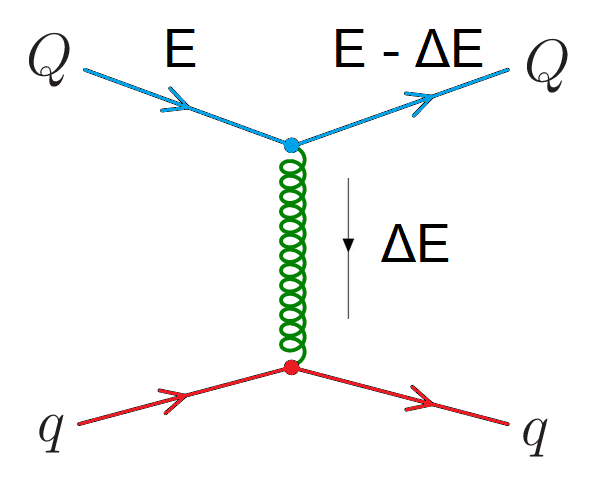
\includegraphics[width=0.35\textwidth]{Figures/Chapter1/Collisional.png}
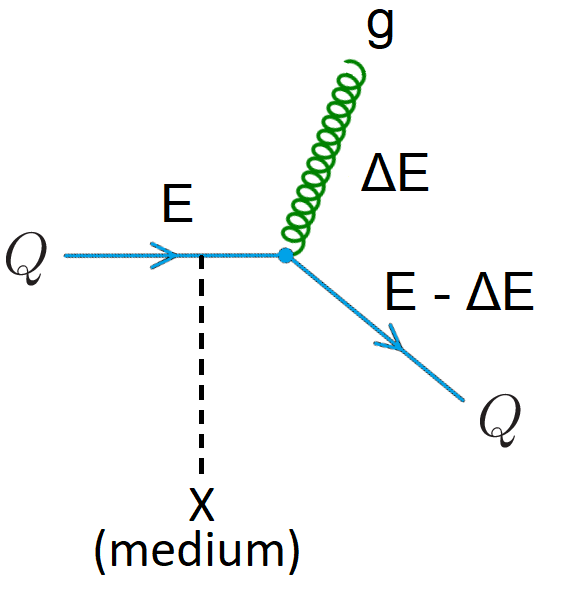
\includegraphics[width=0.35\textwidth]{Figures/Chapter1/Radiative.png}
\caption{The schematic demonstration of the pQCD picture: collisional energy loss (left) and radiative energy loss (right) of heavy quarks in the QGP medium are shown above.}
\label{HQELosspQCD}
\end{center}
\end{figure}   

The other picture, AdS/CFT, takes the strong coupling limit. In this picture, QGP behave like liquid and heavy quarks scatter off the constituents coherently in the QGP medium. The AdS/CFT model applies holographic drag force \cite{ADSCFTDrag} to calculate the energy loss of heavy quark \cite{HQHoloELoss} in the QGP medium

 \begin{figure}[hbtp]
\begin{center}
\includegraphics[width=0.45\textwidth]{Figures/Chapter1/ADSCFT.png}
\caption{The schematic demonstration of ADS/CFT picture: a quark lose energy in the QGP medium holographically due ADS/CFT drag force.}
\label{ADCCFT}
\end{center}
\end{figure}  

%The energy of a heavy quark in the QGP medium according to AdS/CFT calculations is given by:

In the pQCD picture, as $p_T \rightarrow \infty$, similar to electron Bremsstrahlung via QED radiation in the matter \cite{Brems}, for a heavy quark traveling through the QGP medium, its radiative energy loss via soft gluon radiation will dominate. The soft gluon radiation spectrum by a parton in the QGP medium is given by \cite{DEADCONE}

\begin{equation}
dP = \frac{\alpha_S C_{F}}{\pi} \frac{d\omega}{\omega}\frac{k_{\perp}^2 dk_{\perp}^2}{(k_{\perp}^2  + \omega^2\theta_0^2)^2}
\end{equation}

Where 

\begin{equation}
\theta_0 \equiv \frac{m}{E}
\end{equation}

Here, $\omega$ is the energy of the gluon and $k_{\perp}$ is the transverse momentum of the gluon, $C_F$ is color factor (Casimir) which is $3$ for gluons with one color and one anti-color charges and $4/3$ for quarks with one color charge. From Equation 1.78 above, a suppression of radiation at a small angle $0 < \theta < \theta_0$ is expected. This is effect is known as the dead cone phenomenon \cite{DEADCONE}. In Equation 1.79, that as $m$ increases, the dead cone angle $\theta_0 = \frac{m}{E}$ will decrease as the parton mass increases. Figure \ref{DeadConePic} schematically shows a charm quark radiate gluon in the medium with a dead cone in the small angle:

 \begin{figure}[hbtp]
\begin{center}
\includegraphics[width=0.85\textwidth]{Figures/Chapter1/CharmDeadCone.png}
\caption{The schematic demonstration of a charm quark radiation is shown above. A suppression in small angle due to the dead cone effect in the QGP medium is highlighted.}
\label{DeadConePic}
\end{center}
\end{figure}  

Since we have the follow mass hierarchy for quarks and gluons:

\begin{equation}
m_g < m_q < m_c < m_b
\end{equation}

We should expect the energy loss to follow

\begin{equation}
\Delta E_g > \Delta E_q > \Delta E_c >  \Delta E_b
\end{equation}

We call the inequality above to be the flavor dependence of energy loss, which is an important feature of heavy quark energy loss mechanism in the QGP medium. The studies of heavy quark energy loss mechanism in QGP will help us determine the fundamental jet transport coefficient $\hat q$ that characterizes the scattering power of the medium \cite{HQReview}. which relates to the mean free path and the momentum diffusion coefficient of heavy quarks \cite{qhatStudy}. The determination of $\hat q$ will be crucial for us decipher the inner workings of the QGP \cite{JetTransProbe}.

\subsection{Heavy Quark Hadronization}

After heavy quarks traverse through the medium, it will hadronize into heavy flavor hadrons, which could be fully reconstructed from their final state decay products in experiments. As described in Section 1.2.7, in general, hadronization is non-perturbative. Considering heavy quark dynamics and apply hadronization models, physicists develop theoretical models to describe heavy quark hadrochemistry. Below, I will present three model candidates, the Texas A\&M University (TAMU) Model \cite{TAMUModel}, the model developed from Cao et. al. \cite{CaoSunKo}, and the Equal Velocity Recombination (EVR) model \cite{EVR} to describe beauty quark production and hadronization in vacuum:


\subsubsection{TAMU Model}

The TAMU Model uses a thermodynamic T-matrix formulism in terms of ``ladder diagrams'' to compute the heavy quark in-medium scattering amplitude and determine the non-perturbative transport parameters $A_i$ and $B_{ij}$ in the Planck-Fokker equation shown in Eq 1.81 \cite{TAMUModel}. Figure \ref{LadderDiagram} shows schematically the ``ladder diagram'' describing the dynamic evolution of a heavy quark in the QGP medium 

 \begin{figure}[hbtp]
\begin{center}
\includegraphics[width=1.0\textwidth]{Figures/Chapter1/LadderDiagram.png}
\caption{The ladder diagram used by the TAMU model to describe heavy quark diffusion in the QGP medium is shown schematically above.}
\label{LadderDiagram}
\end{center}
\end{figure}  

The input of T-matrix uses a lattice QCD potential \cite{LQCDTAMU} corrected with relativistic effects to model the non-perturbative interaction between heavy quarks and partons in the medium and make it consistent with heavy flavor spectroscopy in vacuum to determine the thermal relaxation rate coefficient $A_i(p,T)$. Only elastic collisional energy loss is included in the calculation. Resonance recombination model of heavy quark with a light quark nearby is applied to describe heavy quark hadronization \cite{RRM1}. A FONLL fragmentation hadronization treatment is implemented for the partons that do not coalesce. Finally, effective hadronic scattering amplitudes are used to model heavy flavor hadronic rescattering with other hadrons before kinetic freez-out stage. The background parton composition and kinematics are modeled by the standard hydrodynamic simulations of the bulk medium in nuclear collisions

\subsubsection{Cao, Sun, Ko Model}

The Cao, Sun, Ko Model employs an advanced Langevin-hydrodynamics approach \cite{CaoLH1,CaoLH2} incorporating both elastic and inelastic energy loss of heavy quarks inside the dynamical QGP medium. The equation below schematically shows relativistic Langevin equation to simulate the dynamics of heavy quarks in the QGP medium


\begin{equation}
\Delta \vec{p} = - \gamma \frac{T^2}{M} \vec{p} \Delta t + \vec{\xi}(t) 
\end{equation}

And

\begin{equation}
\Delta \vec{x} = - \frac{\vec{p}}{E} \Delta t
\end{equation}

The noise is modeled by the Gaussian diffusion function 

\begin{equation}
P(\vec{\xi}) \propto \exp[\frac{\vec{\xi}^2}{2D_p \Delta t}]
\end{equation}

The dimensionless $\gamma$ factor is defined as

\begin{equation}
\gamma = \frac{M}{\tau_{HQ} T^2}
\end{equation}


The Cao, Sun, Ko Model uses a comprehensive coalescence model with strict energy-momentum conservation and PYTHIA fragmentation simulation (Peterson Fragmentation Function)\cite{PYTHIAFrag} with the default Peter fragmentation function. The coalescence probability is determined from resonant scattering rate of heavy quarks in the QGP according to the resonant recombination model \cite{RRM1,RRM2}. In this model, if heavy quarks do not coalesce, they will hadronize via fragmentation mechanism. The hadron interactions in the freeze-out stage are model with UrQMD developed by the Duke theory group. 



 
\subsubsection{EVR Model}

In this model, the transverse momentum distribution of initially produced heavy quark is calculated by FONLL \cite{EVR}. The jet quenching effect in heavy-ion collisions is considered according to $R_{AA}$ measurement of $B^+$. The transverse momentum distributions of light-flavor quarks are obtained from data of light hadrons in the model. This model is particular designed to study low $p_T$ and mid-rapidity charm quarks produced at the LHC energy. It considers the equal-velocity combination of bottom quark with light-flavor anti-quarks  to form B mesons, a framework based on of co-moving quark recombination model (QCM).


In addition to TAMU, Cao, Sun, Ko, and EVR Models, there are many other theoretical models attempting to describe heavy quark hadrochemistry in heavy-ion collisions. A complete list of heavy quark hadrochemistry models is compiled in the heavy flavor review paper \cite{HQRaff}. Nevertheless, due to the large discrepancies among different hadronization models, our ability to interpret the heavy flavor data is significant limited. Therefore, heavy-ion experimentalists precisely measure heavy flavor physics observables with different species and over broad kinematic ranges and provide constrains for models to reduce the theoretical uncertainties in hadronization.


\iffalse



\subsection{Experimental Observables}

Therefore, physicists propose many experimental observables to study open heavy flavor physics and test theoretical models in heavy ion collisions. Traditionally, heavy flavor hadron $v_2$, $R_{AA}$, and yield ratio are extensively studied. 

\textbf{Heavy Quark Diffusion: $v_2$}

In the QGP medium, heavy quark diffused by the color force and multiple scatter with medium constituents, which could generate sizable azimuthal anisotropy $v_2$ \cite{HQReview}. Experimentally, we scale the $v_2$ and the hadron kinetic energy $K_T = \sqrt{m^2 + p_T^2} - m^2$ of heavy quarks with $n_q$ according to the Number of Constituent Quark (NCQ) Scaling in quark coalescence model \cite{NCDScaling}. Figure \ref{HQV2} shows the comparison of the $v_2/n_q$ as a function of $K_T/n_q$ of $D^0$ ($c\bar u$) meson with light flavor hadrons with STAR experiments at RHIC \cite{STARD0v2} and the CMS experiment at LHC \cite{CMSD0v2}.


\begin{figure}[hbtp]
\begin{center}
\includegraphics[width=0.50\textwidth]{Figures/Chapter1/STARv2.png}
\includegraphics[width=0.485\textwidth]{Figures/Chapter1/CMSv2.png}
\caption{The NCQ scaled $D^0$ $v2/n_q$ vs $K_T/n_q$ and the comparison light hardons measured by the STAR experiment at RHIC (left) and the CMS experiment at LHC (right) are shown above.}
\label{HQV2}
\end{center}
\end{figure}   

We could see a reasonably good NCQ scaling behavior of $D^0$ meson with other light flavor hadrons, which suggests sizable collectivity of charm quarks in the QGP medium.

\textbf{Heavy Quark Energy Loss Mechanism: $R_{AA}$}

As we mentioned previously, the nuclear modification factor $R_{AA}$ of heavy flavor hadrons as a function of $p_T$ could quantify the energy loss of quarks via the shift of the $p_T$ spectra to the left in $AA$ collisions compared to $pp$ collisions. Figure \ref{HQRAA} $R_{AA}$ heavy and flavor hadrons measured with experiments at RHIC and LHC.

\begin{figure}[hbtp]
\begin{center}
\includegraphics[width=0.47\textwidth]{Figures/Chapter1/STARRAA.eps}
\includegraphics[width=0.47\textwidth]{Figures/Chapter1/CMSRAA.png}
\caption{The $D^0$ $R_{AA}$ vs $p_T$ with the STAR experiment in 0 - 10\%, 10 - 40\%, and 40 - 80\% centrality at RHIC and the $D^0$, $B^+$, non-prompt $J/\psi$ and charged hadrons $R_{AA}$ vs $p_T$ at at 0 - 100\% centrality with the CMS experiment at LHC are shown above.}
\label{HQRAA}
\end{center}
\end{figure}   

We could see that $R_{AA}$ of $D^0$ and $B^+$ are both below 1, which suggest charm and beauty quarks lose a significant fraction of energy to the QGP medium. As $p_T$ increases, the $R_{AA}$ of light and heavy flavor hadrons converge to the same value and approach 1, which Lorentz $\gamma$ factor come into play where the mass of the hadron become irrelevant. In addition, the CMS results above indirectly agree with the expectation of the flavor dependence of energy loss: $R_{AA}^{h} < R_{AA}^{D} < R_{AA}^{B} < 1$. With both $R_{AA}$ and $v_2$, we can constrain theoretical models and understand the interaction mechanism of heavy quarks with the QGP medium.

\textbf{Heavy Quark Hadronization: $H_s/H^0$ and $\Lambda_{Q}/H^{0}$}

According to the theoretical reviews of heavy quarks hadrochemistry in heavy-ion collisions \cite{StrangetoLight,BaryontoMeson}, the strange-to-non-strange meson ($H_s/H^0$) and baryon-to-meson ($\Lambda_{Q}/H^{0}$) ratios are excellent observables to test hadronization models. Figure \ref{HadroPlotCharm} shows the fully reconstructed $\Lambda_C^+/D^0$ ratio measured by the STAR and CMS experiments

\begin{figure}[hbtp]
\begin{center}
\includegraphics[width=0.52\textwidth]{Figures/Chapter1/STARLambdaCD0.png}
\includegraphics[width=0.47\textwidth]{Figures/Chapter1/ALICELambdaCD0}
\caption{The fully reconstructed $\Lambda_C^+/D^0$ ratio in pp and heavy-ion collisions measured by the STAR experiment at RHIC (left) and the CMS experiment at LHC (right) are shown above.}
\label{HadroPlotCharm}
\end{center}
\end{figure}   

We can see that in general, $\Lambda_C^+/D^0$ ratio in heavy-ion collisions lies above its ratio in $pp$ collisions. Moreover, there are many different theoretical predictions agree reasonably well with the experiments due to the large uncertainties. More precise $\Lambda_C^+/D^0$ measurements will be desired in order to constrain theoretical models.

In addition to $v_2$, $R_{AA}$, and $\Lambda_{Q}/H^{0}$, some modern observables with more differentiation such as the hadron-hadron correlation and heavy flavor jet substructure measurements have been recently carried out \cite{DDbar,DJet}. 

Hence, with the motivation to understand the hadronization mechanism of heavy quarks and investigate the inner workings of the QGP, I propose to carry out open heavy flavor physics measurements. In this thesis, I will focus on the measurement of the experimental observable $B^0_s/B^+$ ratio from fully reconstructed $B^0_s$ and $B^+$ mesons (and their anti-particles) via decay channels of $B^0_s \rightarrow J/\psi \phi \rightarrow \mu^+ \mu^- K^+ K^-$ and $B^0_s \rightarrow J/\psi K^+ \rightarrow \mu^+ \mu^- K^+$ in pp and PbPb collisions with the CMS experiment at the LHC to study the beauty production and hadronization mechanism in vacuum and QGP. 



\fi
